Przedmiotem rozważań w rozdziale 5 są wyniki analizy wybranych modeli zarządzania podatnościami otrzymane dla trzech niezależnych środowisk teleinformatycznych. Środowiska teleinformatyczne omówione szczegółowo w rozdziale 3 są zróżnicowane aby ułatwić omówienie wad i zalet analizowanych modeli zarządzania podatnościami, które zaproponowano w rozdziale 1. Nie oznacza to jednak, że zaproponowane w rozdziale 2 rozwiązania mogą być wykorzystane tylko i wyłącznie w analizowanych środowiskach teleinformatycznych. Na podstawie otrzymanych wyników można bowiem wyciągnąć wnioski o charterze ogólnym stosowalne dla dowolnego środowiska teleinformatycznego. Wybrane środowiska teleinformatyczne różnią się liczbą wykrytych podatności, a także liczbą podatności, dla których znana jest ocena bazowa dla standardu CVSS 2.0 oraz 3.x. Dodatkowa różnica pomiędzy środowiskami teleinformatycznymi odnosi się do informacji otrzymanych od administratorów. Dla środowiska teleinformatycznego A, oprócz podania danych na temat wykrytych podatności, administrator przekazał informacje dotyczące ustawień parametrów środowiskowych $CIA$. Dla środowiska teleinformatycznego B otrzymano tylko raport z wykrytymi podatnościami za pomocą oprogramowania Nessus. Dla środowiska teleinformatycznego C otrzymano raport z podatnościami wykrytymi za pomocą oprogramowania Nessus oraz ogólne informacje dotyczące wag skanowanych zasobów. Wyniki otrzymane dla tychże trzech różnych i niezależnych środowisk teleinformatycznych wykorzystano w tym rozdziale do analizy modeli procesu zarządzania podatnościami (Rozdział \ref{sec:modele-zarzadzaia-podatnosciami}). 

\bigbreak
Dla każdego rozpatrywanego środowiska wyniki analizy uporządkowano w następujący sposób. Najpierw porównano modele zarządzania podatnościami, które wykorzystują standard CVSS 2.0 (Rysunek \ref{fig:chapter1:vm-model-cvss2}, \ref{fig:chapter1:vm-model-cvss2e}). W tym celu do oceny bazowej CVSS 2.0 dodano dane środowiskowe, a następnie przeanalizowano liczbę oraz zakres zmian w kategoriach podatności w porównaniu z oceną bazowa CVSS 2.0. Jak wykazano w tym rozdziale w oparciu o przeprowadzoną analizę, model zarządzania podatnościami, który wykorzystuje ocenę środowiskową CVSS 2.0 ma istotną wadę. Wada ta polega na tym, że parametr $TD$, który służy do ustalania liczby systemów wrażliwych na daną podatność, znacząco zaniża oceny wszystkich wykrytych podatności. Dlatego też ocena środowiskowa CVSS 2.0 nie jest dokładną miarą bezpieczeństwa infrastruktury teleinformatycznej. Konieczne było zatem rozważenie modelu zarządzania podatnościami, który opiera się na standardzie CVSS 3.x. Dokonano więc analizy modelu zarządzania podatnościami, która oprócz oceny bazowej CVSS 3.x uwzględnia także dane środowiskowe. Następnie ponownie przeanalizowano liczbę oraz zakres zmian w kategoriach podatności dla takiego modelu zarządzania podatnościami. Należy jednak zauważyć, ze implementacja modelu zarządzania podatnościami, które wykorzystuje standard CVSS 3.x okazała się trudna w praktyce. Jest bowiem wiele podatności, dla których znana jest tylko ocena bazowa CVSS 2.0. Wykonanie priorytetyzacji za pomocą modeli zarządzania podatnościami według standardu CVSS 3.x (Rysunek \ref{fig:chapter1:vm-model-cvss3}, \ref{fig:chapter1:vm-model-cvss3e}) nie było zatem w pełni możliwe z powodu braku ocen bazowych CVSS 3.x dla niektórych z wykrytych podatności. Problem ten rozwiązano przez zastosowanie metod uczenia maszynowego, które wykorzystano do przeprowadzenia konwersji oceny bazowej ze standardu CVSS 2.0 do standard 3.x, w przypadku podatności, dla których znana jest jedynie ocena bazowa CVSS 2.0. Szczegóły tej konwersji są opisane w w rozdziale \ref{sec:ml}. Po przeprowadzeniu konwersji możliwa była pełna implementacja modelu zarządzania podatnościami dla standardu 3.x i oszacowanie liczby oraz zakresu zmian w poszczególnych kategoriach podatności. Ponadto dla każdego środowiska teleinformatycznego oraz analizowanego modelu zarządzania podatnościami oszacowano liczbę roboczogodzin wymaganych do usunięcia wszystkich podatności z wyjątkiem podatności o krytyczności niskiej. W tym celu skorzystano z równań wyprowadzonych w rozdziale \ref{sec:modele-ewaluacji-efektywnosci}. Otrzymane wyniki pozwoliły na wyciągnięcie istotnych wniosków dotyczących wpływu danych środowiskowych na ocenę bazową CVSS.

\bigbreak
W rozdziale 5 przeprowadzono także analizę skalowalności opracowanego oprogramowania. Czas oczekiwania na wyniki priorytetyzacji podatności jest niezwykle istotny, ponieważ jest to również czas ekspozycji środowiska teleinformatycznego na zagrożenia wynikające z możliwości wykorzystania danej podatności przez atakującego. Redukcja czasu oczekiwania na wyniki priorytetyzacji podatności jest istotna także dlatego, że wykrywane jest coraz więcej podatności, ponadto środowiska teleinformatyczne mogą podlegać szybkim zmianom. Czas reakcji jest zatem krytycznym parametrem, gdy rozważa się bezpieczeństwo zasobów systemu teleinformatycznego. Dlatego też w ramach przeprowadzonych badań oszacowano czas trwania obliczeń w zależności od liczby modułów obliczeniowych oraz liczby przetwarzanych danych. Analiza ta została przeprowadzona w środowisku opisanym w rozdziale \ref{sec:desc_skalowalnosc}, ponieważ właściciele zasobów udostępniających dane dotyczące wykrytych podatności nie wyrazili zgody na przetwarzanie danych w chmurze.

\bigbreak
Rozdział 5 składa się z trzech części. W pierwszej części omówione zostały wyniki analizy skalowalności opracowanego rozwiązania w środowisku chmurowym. W części drugiej, omówione zostały wyniki analizy otrzymane dla środowisk teleinformatycznych przedstawionych w rozdziałach \ref{sec:desc_a}, \ref{sec:desc_b}, \ref{sec:desc_c}. Część trzecia poświęcona jest podsumowaniu uzyskanych wyników.

%%%%%%%%%%%%%%%%%%%%%%%%%%%%%%%%%%%%%%%%%%%%%%%%

%%%%%%%%%%%%%%%%%%%%%%%%%%%%%%%%%%%%%%%%%%%%%%%%
\section{Analiza czasu obliczeń obliczeń dla dużej ilości danych}
\label{sec:analiza_skalowania}
Właściciele zasobów, od których pozyskano informacje na temat podatności znajdujących się w ich infrastrukturze (Rozdziały \ref{sec:desc_a}, \ref{sec:desc_b}, \ref{sec:desc_c}) nie wyrazili zgody na przetwarzanie danych w chmurze. Dlatego w celu przeprowadzenia analizy, skalowalności rozwiązania oraz pomiaru czasu wykonywania obliczeń stworzono środowisko wirtualne zawierające 2 110 adresy IP. Dla każdego adresu IP przydzielono w sposób losowy podatności z publicznie dostępniej bazy podatności NVD \cite{booth2013national}. W rezultacie otrzymano wirtualne środowisko zawierające 168 940 podatności, z czego 3 008 podatności było unikalnych, to znaczy, że wystąpiło tylko raz na jednym adresie IP. Następnie przygotowano środowisko chmurowe, które wykorzystuje konfiguracje opisaną w rozdziale \ref{sec:desc_skalowalnosc} oraz przygotowano 12 scenariuszy testowych $P_0$ - $P_{12}$, dla których zmierzono czas trwania obliczeń:
\begin{description}
    \item $P_0$ — obliczenie oceny środowiskowej CVSS 2.0 i CVSS 3.x dla stworzonego środowiska wirtualnego,
    \item $P_1$ — obliczenie oceny środowiskowej CVSS 2.0 i CVSS 3.x dla stworzonego środowiska wirtualnego, przy czym dla 10\% zasobów (adresów IP) zmieniono składową środowiskową wektora CVSS (jeden z parametrów $CIA$),
    \item $P_2$ — obliczenie oceny środowiskowej CVSS 2.0 i CVSS 3.x dla stworzonego środowiska wirtualnego, przy czym dla 20\% zasobów (adresów IP) zmieniono składową środowiskową wektora CVSS (jeden z parametrów $CIA$),
    \item $P_3$ — obliczenie oceny środowiskowej CVSS 2.0 i CVSS 3.x dla stworzonego środowiska wirtualnego, przy czym dla 30\% zasobów (adresów IP) zmieniono składową środowiskową wektora CVSS (jeden z parametrów $CIA$),
    \item $P_4$ — obliczenie oceny środowiskowej CVSS 2.0 i CVSS 3.x dla stworzonego środowiska wirtualnego, przy czym zmniejszono liczbę zasobów (adresów IP) o 10\%,
    \item $P_5$ — obliczenie oceny środowiskowej CVSS 2.0 i CVSS 3.x dla stworzonego środowiska wirtualnego, przy czym zmniejszono liczbę zasobów (adresów IP) o 20\%,
    \item $P_6$ — obliczenie oceny środowiskowej CVSS 2.0 i CVSS 3.x dla stworzonego środowiska wirtualnego, przy czym zmniejszono liczbę zasobów (adresów IP) o 30\%,
    \item $P_7$ — obliczenie oceny środowiskowej CVSS 2.0 i CVSS 3.x dla stworzonego środowiska wirtualnego, przy czym zwiększono liczbę podatności o 10\%,
    \item $P_8$ — obliczenie oceny środowiskowej CVSS 2.0 i CVSS 3.x dla stworzonego środowiska wirtualnego, przy czym zwiększono liczbę podatności o 20\%,
    \item $P_9$ — obliczenie oceny środowiskowej CVSS 2.0 i CVSS 3.x dla stworzonego środowiska wirtualnego, przy czym zwiększono liczbę podatności o 30\%,
    \item $P_{10}$ — obliczenie oceny środowiskowej CVSS 2.0 i CVSS 3.x dla stworzonego środowiska wirtualnego, przy czym zmniejszono liczbę podatności o 10\%,
    \item $P_{11}$ — obliczenie oceny środowiskowej CVSS 2.0 i CVSS 3.x dla stworzonego środowiska wirtualnego, przy czym zmniejszono liczbę podatności o 20\%,
    \item $P_{12}$ — obliczenie oceny środowiskowej CVSS 2.0 i CVSS 3.x dla stworzonego środowiska wirtualnego, przy czym zmniejszono liczbę podatności o 30\%,
\end{description}

\bigbreak
Każdy scenariusz testowy powtórzono trzykrotnie, a następnie wyznaczono średnią wartość czasu obliczeń. Za każdym razem, gdy scenariusz testowy był powtarzany, opracowane oprogramowanie było restartowane w celu wykluczenia wpływu automatycznych optymalizacji wykonywanych przez komponenty oprogramowania wytworzone przez firmy zewnętrzne. Na przykład oprogramowanie Elasticsearch ma zaimplementowany mechanizm optymalizacji czasu wykonywania zapytań, który wykorzystuje pamięć podręczną serwera (ang. cache). Mechanizm ten automatycznie redukuje czas obliczeń, gdy wykonywane zapytania są do siebie podobne. Jeśli opracowane oprogramowanie nie byłoby restartowane, to włączyłby się mechanizm optymalizacji oprogramowania Elasticsearch i wpłynęłoby to na czas obliczeń.

\bigbreak
Rysunek \ref{fig:chapter6:p_process} przedstawia średni czas trwania obliczeń w zależności od liczby aktywnych modułów obliczeniowych dla wybranych scenariuszy testowych $P_0$ - $P_{12}$. Wyniki przedstawione na rysunku \ref{fig:chapter6:p_process} potwierdzają, że dla każdego rozpatrywanego scenariusza testowego możliwe jest skrócenie czasu obliczeń poprzez zwiększenie liczby aktywnych modułów obliczeniowych. Dla scenariuszy testowych ($P_1$, $P_2$, $P_3$), w których rozważana jest zmiana parametrów środowiskowych $CIA$, odnotowano zwiększenie czasu obliczeń. Związane to jest ze zwiększoną liczbą operacji aktualizacji danych podczas pobierania informacji z bazy danych zasobów Ralph. Dla scenariuszy testowych ($P_4$, $P_5$, $P_6$), w których rozważane jest zmniejszenie liczby adresów IP posiadających znane podatności, obserwuje się skrócenie czasu obliczeń. Związane jest to ze znacznym zmniejszeniem ilości danych, dla których potrzeba wykonać obliczenia, ponieważ każdy adres IP ma przypisaną różną liczbę podatności. Na przykład usunięcie adresu IP 192.168.0.123 z środowiska wirtualnego powoduje usunięcie 100 podatności. Dla przypadków testowych ($P_7$, $P_8$, $P_9$), w których rozważane jest zwiększenie liczby podatności w środowisku wirtualnym, odnotowano największy wzrost czasu obliczeń. Natomiast dla przypadków testowych ($P_{10}$, $P_{11}$,$P_{12}$), w których rozważono usunięcie podatności ze środowiska wirtualnego, odnotowano największe skrócenie czasu obliczeń. Związane jest to z potrzebą wykonania ponownych obliczeń parametru $TD$, który jest parametrem oceny środowiskowej CVSS 2.0. Parametr środowiskowy $TD$ służy do ustalania liczby systemów wrażliwych na daną podatność. Ponieważ dla oceny środowiskowej CVSS 3.x nie ma żadnego parametru dotyczącego dystrybucji podatności, nie jest ona ponownie obliczana. We wszystkich rozważanych przypadkach największe skrócenie czasu obliczeń obserwuje się po dodaniu 2 aktywnego modułu obliczeniowego (obniżenie czasu obliczeń o około 45\%), ponieważ ilość danych, która musi zostać obliczona rozkładana jest prawie równomiernie na dwa moduły obliczeniowe. Optymalna liczba aktywnych modułów obliczeniowych dla wykorzystanego środowiska wirtualnego wynosi 5 (obniżenie czasu obliczeń o 66\%). Największe skrócenie czasu obliczeń o 70\% uzyskano dla 6 aktywnych modułów obliczeniowych oraz scenariusza testowego $P_{12}$. Związane jest to z najmniejszą ilością danych, które muszą zostać przetworzone przez jeden moduł obliczeniowy.

\begin{figure}[!ht]
\centering
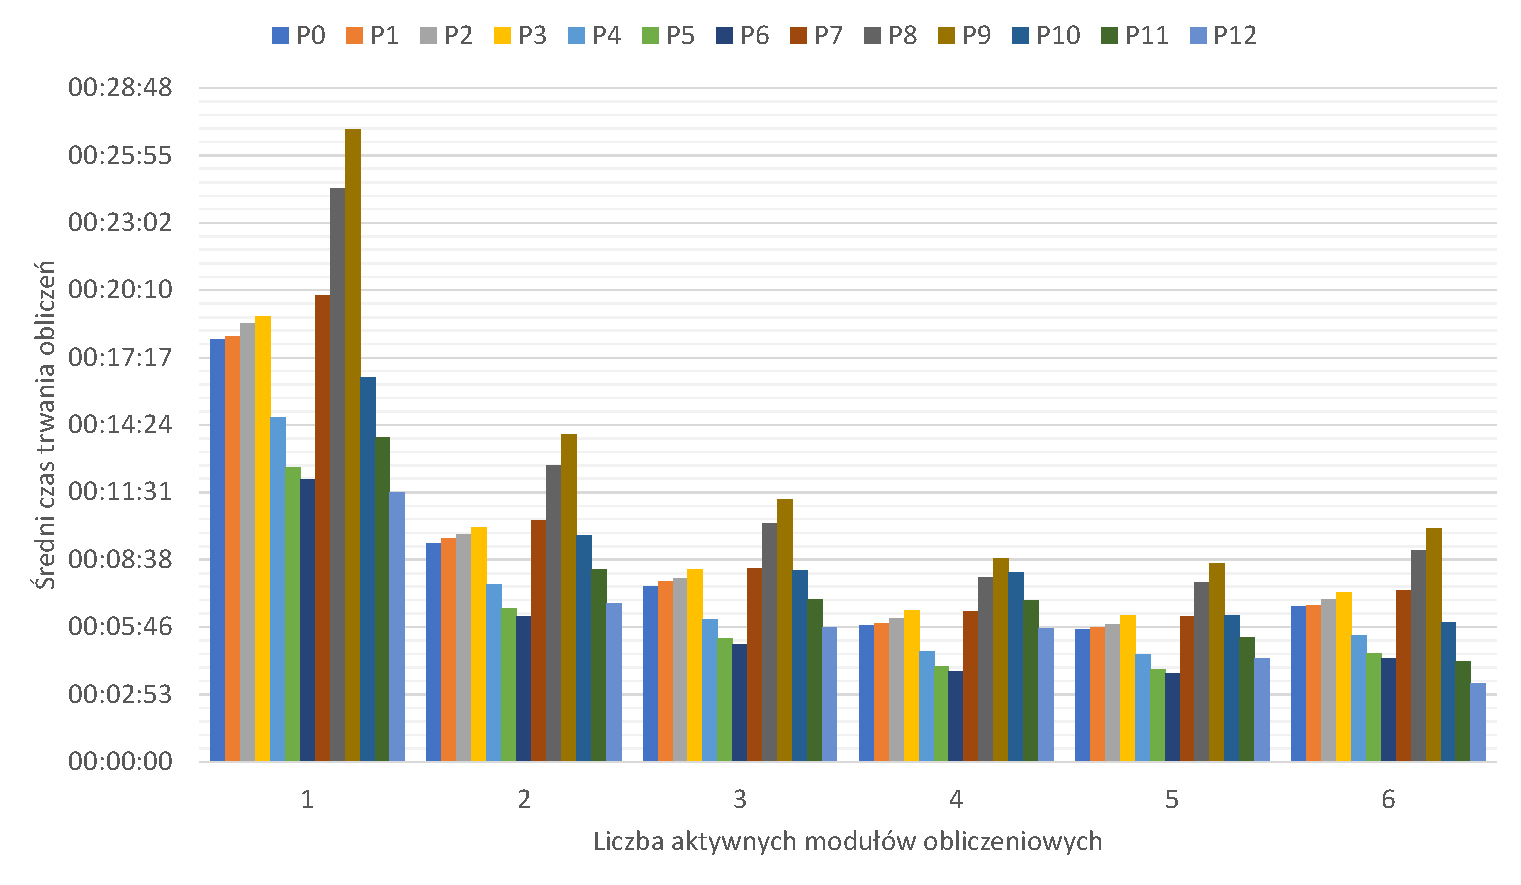
\includegraphics[width=.9\textwidth]{Chapters/Eksperymenty/scaling_results/p_proces.pdf}
\caption{Średni czas trwania obliczeń w zależności od liczby aktywnych modułów obliczeniowych dla wybranych scenariuszy testowych $P_0$ - $P_{12}$.}
\label{fig:chapter6:p_process}
\end{figure}


\bigbreak
Przeprowadzona analiza z wykorzystaniem dużej ilości danych w środowisku chmurowym (Rozdział \ref{sec:desc_skalowalnosc}) potwierdziła, że wytworzone oprogramowanie w ramach rozprawy doktorskiej z wykorzystaniem najnowszych technologii, takich jak Docker (Rozdział \ref{sec:docker}) oraz Kubernetes (\ref{sec:k8s}), przystosowane jest do przetwarzania przyrastającej ilości danych. Otrzymane czasy obliczeń dla wszystkich rozpatrywanych przypadków w porównaniu do czasu trwania skanowania oraz naprawy podatności są pomijalne, ponieważ, jak wykazano w rozdziale \ref{sec:desc_env_all}, czas skanowania oraz naprawy podatności liczony jest w godzinach. Na przykład najkrótszy czas skanowania otrzymany został dla środowiska teleinformatycznego A wynoszący 3 godziny. Natomiast czas naprawy podatności, jak przedstawiono w pracy \cite{farris2018vulcon}, mieści się w zakresie od 1 do 9 roboczogodzin. Ponadto opracowane oprogramowanie (Rozdział \ref{sec:scaling}) dla przypadku zwiększenia liczby aktywnych modułów obliczeniowych tylko o jeden, pozwala na zmniejszenie czasu przetwarzania danych aż o 45\%. W pełni zatem uzasadnione jest pominięcie w równaniach \ref{eq:cvss2e}, \ref{eq:cvss3e} czasu trwania wykonywania obliczeń ($T_{VMC}$). Dodatkowo w analizie wyłączono wszystkie możliwe optymalizacje dostarczane przez producentów wykorzystywanego oprogramowania Elasticsearch. W przypadku wykorzystania realnego środowiska z odpowiednio zaplanowaną architekturą możliwe jest otrzymanie jeszcze krótszych czasów obliczeń. Otrzymane wyniki pozwalają na stwierdzenie, że wykorzystując wytworzone oprogramowanie, możliwe jest rozwiązanie problemu przedstawionego w rozdziale \ref{sec:modele-zarzadzaia-podatnosciami}, dotyczącego skalowalności. Mianowicie wytworzone oprogramowanie dostosowane jest do rosnącej ilości napływających danych.

\bigbreak
Podsumowując, można stwierdzić, że dzięki wykorzystaniu zaimplementowanych rozwiązań przedstawionych w rozdziale drugim możliwa była istotna redukcja czasu obliczeń, ponieważ czas skanowania oraz naprawy podatności liczony jest w godzinach. Natomiast dla wszystkich analizowanych środowisk teleinformatycznych czas obliczeń z wykorzystaniem opracowanego oprogramowania wynosił poniżej minuty i nie miał większego wpływu na całościowy czas trwania procesu. Dlatego też w obliczeniach wykorzystujących równania \ref{eq:cvss2e} i \ref{eq:cvss3e}, dotyczących szacowanej liczby roboczogodzin wymaganych do usunięcia istotnych podatności bezpieczeństwa infrastruktury teleinformatycznych, można założyć, że $T_{VMC}$ = 0. W następnym podrozdziale przeprowadzono obliczenia szacowanej liczby roboczogodzin wymaganych do usunięcia istotnych podatności bezpieczeństwa dla trzech wybranych środowisk teleinformatycznych.

%%%%%%%%%%%%%%%%%%%%%%%%%%%%%%%%%%%%%%%%%%%%%%%%

%%%%%%%%%%%%%%%%%%%%%%%%%%%%%%%%%%%%%%%%%%%%%%%%
\section{Analiza zaproponowanych modeli zarządzania podatnościami}
Właściciele zasobów, od których pozyskano informacje na temat podatności znajdujących się w ich infrastrukturze (Rozdziały \ref{sec:desc_a}, \ref{sec:desc_b}, \ref{sec:desc_c}), nie wyrazili zgody na przetwarzanie danych w chmurze. Dlatego w celu przeprowadzenia analizy wykorzystano środowisko badawcze opisane w rozdziale \ref{sec:desc_pio}.

\bigbreak
Sposób przeprowadzenia analizy dla wszystkich środowisk teleinformatycznych wyglądał w następujący sposób:
\begin{enumerate}
    \item wczytanie raportu dotyczącego wykrytych podatności do narzędzia Nessus \cite{beale2004nessus},
    \item wczytanie danych dotyczących kategorii krytyczności dla analizowanego środowiska ICT do bazy inwentaryzacji zasobów Ralph \cite{ralph} (informacje otrzymane od administratorów),
    \item ręczne wymuszenie w panelu administratora wytworzonego na potrzeby pracy VMC, synchronizacji danych,
    \item analiza otrzymanych wyników.
\end{enumerate}

%%%%%%%%%%%%%%%%%%%%%%%%%%%%%%%%%%%%%%%%%%%%%%%%

%%%%%%%%%%%%%%%%%%%%%%%%%%%%%%%%%%%%%%%%%%%%%%%%
\subsection{Analiza dla środowiska teleinformatycznego A}

%%%%%%%%%%%%%%%%%%%%%%%%%%%%%%%%%%%%%%%%%%%%%%%%

%%%%%%%%%%%%%%%%%%%%%%%%%%%%%%%%%%%%%%%%%%%%%%%%
\subsubsection{Analiza wpływu parametrów środowiskowych na ocenę bazową CVSS 2.0}
\label{sec:analiza_cvss2_ev_a}
Rysunek \ref{fig:chapter6:env_a:cvss_2} przedstawia liczbę wykrytych podatności dla każdej kategorii krytyczności według oceny bazowej i środowiskowej CVSS 2.0. Na podstawie wyników pokazanych na rysunku \ref{fig:chapter6:env_a:cvss_2} można stwierdzić, że dla oceny środowiskowej CVSS 2.0 wszystkie podatności zostały przydzielone do kategorii niskiej. Wpływ na to ma parametr $TD$ (Rozdział \ref{sec:td}), który osiągnął maksymalną wartość 13\%, co zostało przedstawione na rysunku \ref{fig:chapter6:env_a:cvss_2_td}. Parametr $TD$ wskazuje procent zasobów wrażliwych na konkretną podatność. Rysunek \ref{fig:chapter6:env_a:cvss_2_td} przedstawia wartość parametru $TD$ dla wykrytych podatności w środowisku teleinformatycznym A. Wpływ pozostałych parametrów środowiskowych na kategorię krytyczności podatności, $CDP$ (Rozdział \ref{sec:cdp}) oraz $CIA$ (Rozdział \ref{sec:cia_desc}) jest niezauważalny, ponieważ parametr $TD$ osiąga maksymalną wartość 13\%. Wyniki przedstawione na rysunku \ref{fig:chapter6:env_a:cvss_2} potwierdzają, że model zarządzania podatnościami, który wykorzystuje ocenę środowiskową CVSS 2.0, ma istotną wadę. Wada ta polega na tym, że parametr $TD$, który służy do ustalania liczby systemów wrażliwych na daną podatność, znacząco zaniża oceny wszystkich podatności. Dlatego też model zarządzania podatnościami oparty o ocenę środowiskową CVSS 2.0 nie jest dokładną miarą bezpieczeństwa infrastruktury teleinformatycznej. Konieczne jest zatem rozważenie modelu zarządzania podatnościami, który opiera się na standardzie CVSS 3.x. Niemniej jednak należy zauważyć, że ocena środowiskowa CVSS 2.0 dostarcza bardzo ważnej informacji dla administratora. Mianowicie jeśli wartość parametru $TD$ jest niska, to w badanym środowisku teleinformatycznym wykryta podatność może zagrozić jedynie niewielkiej liczbie serwerów. Na przykład w środowisku A wykryto podatności, których wykorzystanie możne zagrozić co najwyżej 3 serwerom, tj. 13\% skanowanych zasobów.

\begin{figure}[!ht]
\centering
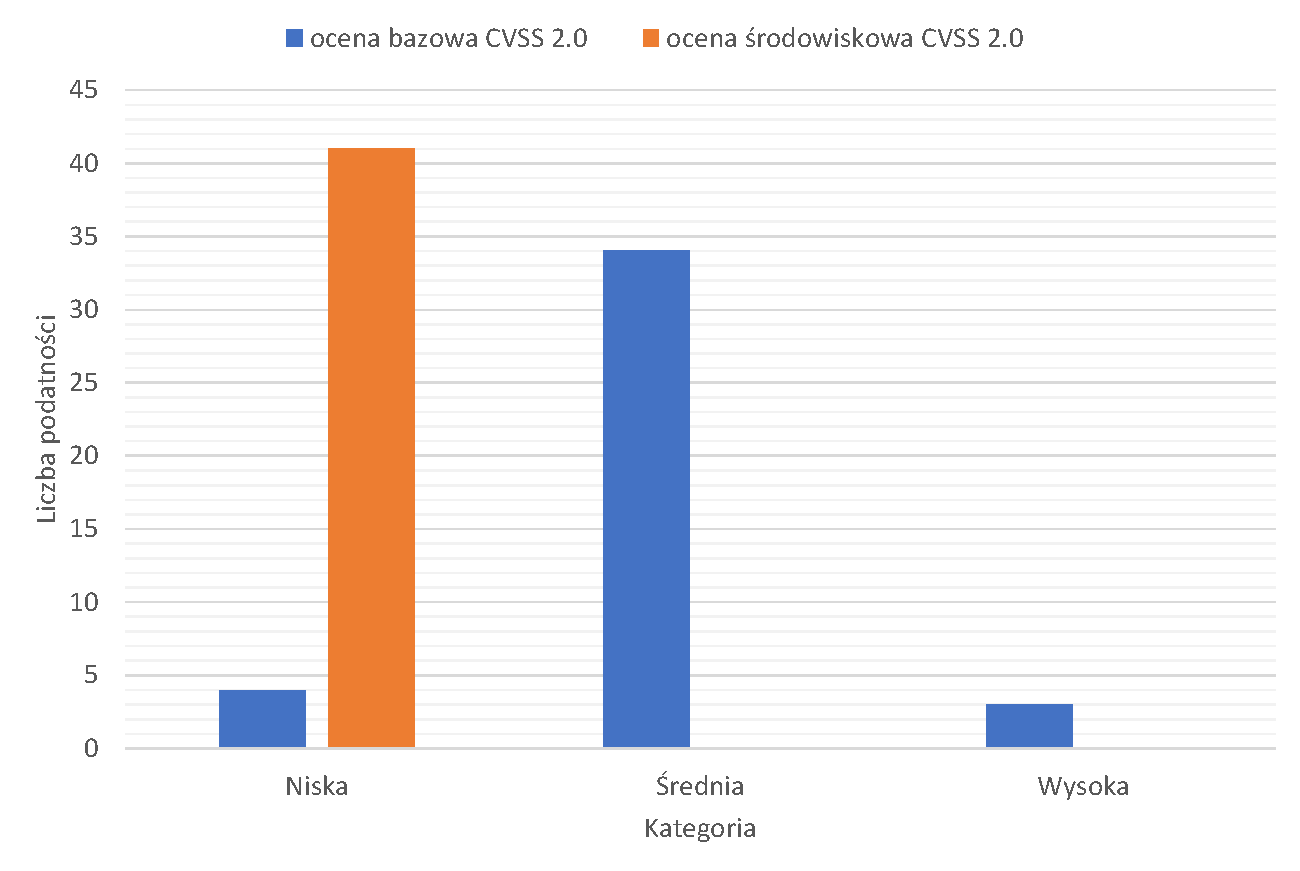
\includegraphics[width=.9\textwidth]{Chapters/Eksperymenty/env_A_results/cvss_2.pdf}
\caption{Liczba wykrytych podatności dla każdej kategorii krytyczności według oceny bazowej i środowiskowej CVSS 2.0 dla środowiska teleinformatycznego A.}
\label{fig:chapter6:env_a:cvss_2}
\end{figure}

\begin{figure}[!ht]
\centering
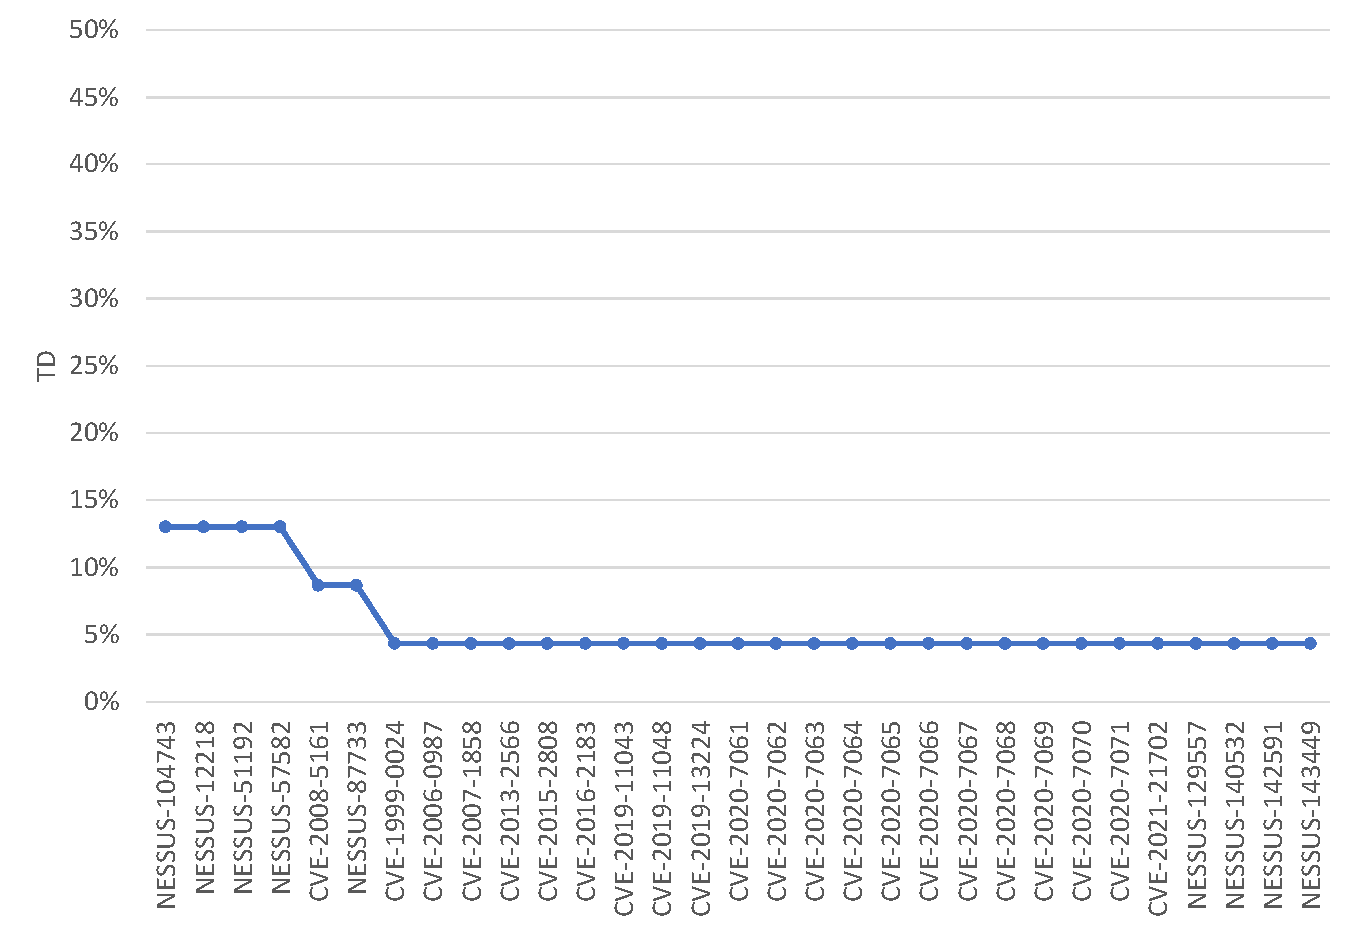
\includegraphics[width=.9\textwidth]{Chapters/Eksperymenty/env_A_results/cvss_2_td_env_a.pdf}
\caption{Wartość parametru $TD$ dla wykrytych podatności w środowisku teleinformatycznym A.}
\label{fig:chapter6:env_a:cvss_2_td}
\end{figure}

\bigbreak
Rysunek \ref{fig:chapter6:env_a:cvss_2_changes} przedstawia liczbę podatności zmodyfikowanych dla danej wartości różnicy pomiędzy oceną bazową a środowiskową CVSS 2.0 w przypadku środowiska teleinformatycznego A. Uwzględnienie parametrów środowiskowych $CIA$, $CDP$, $TD$ spowodowało zmianę wszystkich ocen bazowych CVSS 2.0 w przedziale od -8.9 do -2.4. Brak ocen bazowych niezmodyfikowanych spowodowany jest postacią równania \ref{eq:cvss2_es}, w którym to występuje mnożenie oceny końcowej przez wartość parametru środowiskowego $TD$, w celu otrzymania wartości oceny środowiskowej CVSS 2.0. Z liczby oraz zakresu zmian można wywnioskować, że w zbiorze wykrytych podatności znajdują się zagrożenia, które mogą mieć istotny wpływ na bezpieczeństwo monitorowanego środowiska. 

Zbiór wykrytych podatności w środowisku teleinformatycznym A składa się z dwóch podzbiorów: podatności posiadających obie oceny bazowe (CVSS 2.0 oraz CVSS 3.x) oraz podatności ze znaną jedynie oceną bazową w standardzie CVSS 2.0. W przypadku pierwszego podzbioru podatności posiadają ocenę bazową według standardu CVSS 3.x, w związku z czym priorytetyzacja naprawy zostanie ujęta w procesie zarządzania podatnościami za pomocą modelu \ref{fig:chapter1:vm-model-cvss3e} (Rozdział \ref{sec:proces-zarzadzania-podatnosciami}), ponieważ stosowanie oceny bazowej CVSS 3.x pozwala dokładniej ocenić krytyczność podatności, a zatem skuteczniej oszacować zagrożenia (Rozdział \ref{sec:modele-zarzadzaia-podatnosciami}). W przypadku drugiego podzbioru, który zawiera 14 (34\%) podatności, wykorzystano mechanizm konwersji oceny bazowej CVSS 2.0 do 3.x opisany w rozdziale \ref{sec:ml} w celu umożliwienia wykonania priorytetyzacji za pomocą modelu oceny środowiskowej CVSS 3.x (Rysunek \ref{fig:chapter1:vm-model-cvss3e}).

\begin{figure}[!ht]
\centering
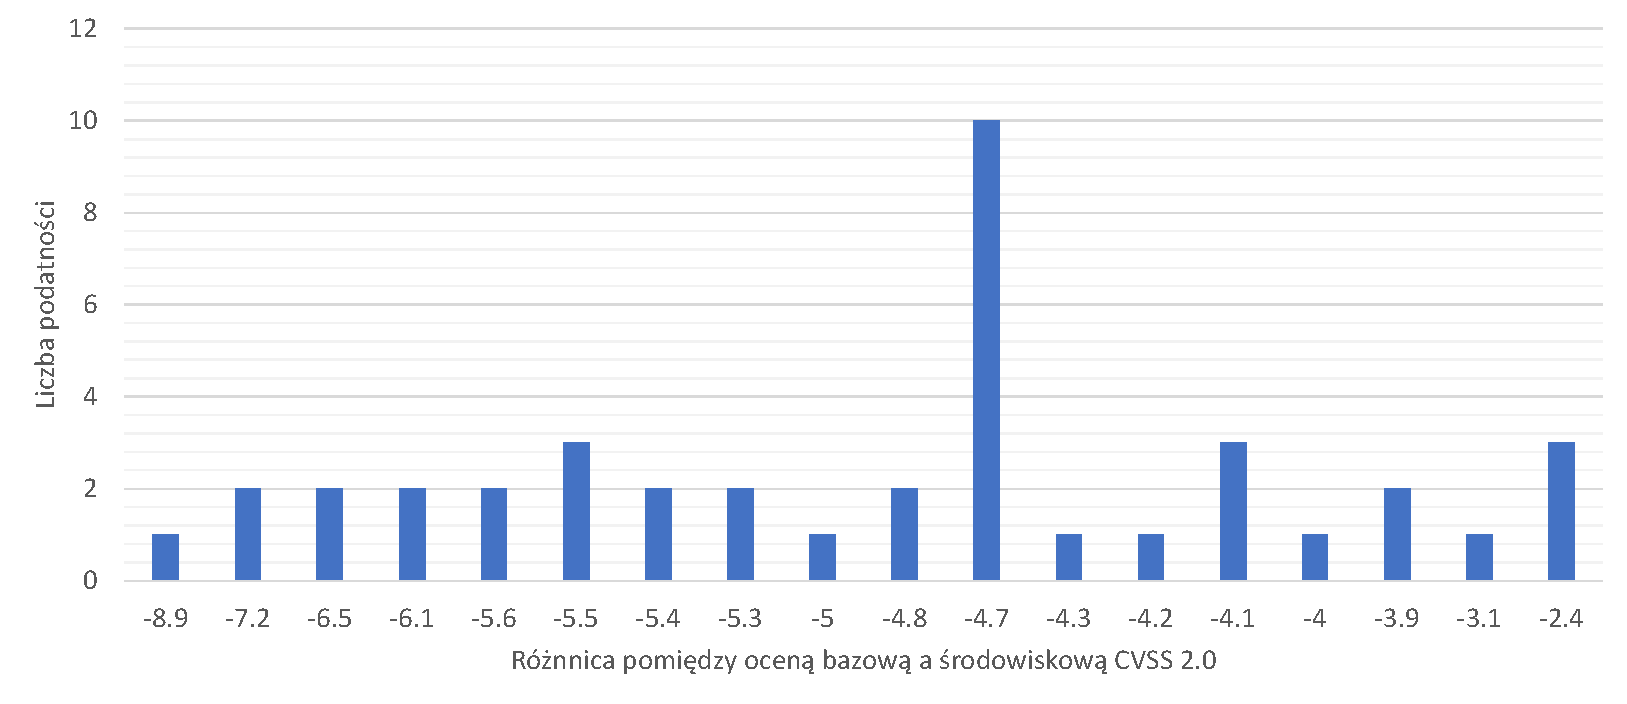
\includegraphics[width=.9\textwidth]{Chapters/Eksperymenty/env_A_results/changes_cvss_2.pdf}
\caption{Liczba podatności zmodyfikowanych dla danej wartości różnicy pomiędzy oceną bazową a środowiskową CVSS 2.0 w przypadku środowiska teleinformatycznego A.}
\label{fig:chapter6:env_a:cvss_2_changes}
\end{figure}

\bigbreak
Tabela \ref{tab:chapter6:env_a:time_results_cvss2} przedstawia liczbę roboczogodzin wymaganą do usunięcia istotnych podatności bezpieczeństwa dla środowiska teleinformatycznego A. W przypadku ocen bazowych CVSS 2.0 szacunkowa liczba roboczogodzin została obliczona za pomocą wzorów: $T_{Base2}$ - \ref{eq:cvss2}, $T_{Base2'}$ - \ref{eq:cvss2prim}. W przypadku oceny środowiskowej CVSS 2.0 szacunkowa liczba roboczogodzin została obliczona za pomocą wzoru \ref{eq:cvss2e}. Wartości dla czasów $T_{Base2}$ obliczone zostały przy założeniu, że administrator musi naprawić tylko podatności o krytyczności wysokiej i średniej, w związku z czym akceptuje ryzyko związane z istnieniem w systemie podatności o krytyczności niskiej. Ponadto należy zauważyć, ze w przypadku priortetyzacji opartej na ocenie bazowej CVSS 2.0, która nie uwzględnia danych środowiskowych wśród podatności sklasyfikowanych jako podatności o krytyczności niskiej mogą się znajdować podatności o wyższej krytyczności, na przykład wysokiej. Wartości czasów $T_{Base2'}$ obliczone zostały zatem przy założeniu, że w celu zapewnienia bezpieczeństwa systemu administrator musi naprawić wszystkie podatności, ponieważ (jak opisano szczegółowo w rozdziale \ref{sec:wplyw_cvss2}) nie ma pewności czy podatność z otrzymaną oceną bazową CVSS 2.0 zachowa tę ocenę po uwzględnieniu danych środowiskowych. Natomiast wartości dla czasów $T_{Env2}$ obliczone zostały przy założeniu, że wszystkie oceny podatności zostały sklasyfikowane dokładnie (Rozdział \ref{sec:modele-zarzadzaia-podatnosciami}). Gdy porówna się szacowane liczby roboczogodzin otrzymane dla $T_{Base2}$ z $T_{Base2'}$, można zauważyć wzrost szacowanej liczy roboczogodzin dla wszystkich rozpatrywanych przypadków ($T_{FIX_{MIN}}$, $T_{FIX_{AVERAGE}}$, $T_{FIX_{MAX}}$), który wynosi 10.4\%. Ponadto można zaobserwować, że naprawienie wszystkich podatności według otrzymanej priorytetyzacji za pomocą oceny bazowej CVSS 2.0 redukuje ryzyko nienaprawienia podatności niedoszacowanej z 10\% do 0\%. Gdy porównamy otrzymane wyniki dla $T_{Base2}$ i $T_{Env2}$, można zauważyć, że średni zysk w postaci obniżenia szacowanej liczby roboczogodzin dla wszystkich rozpatrywanych przypadków wynosi 95.8\%. Wykorzystanie priorytetyzacji za pomocą oceny środowiskowej CVSS 2.0 pozwala na obniżenie ryzyka związanego z nienaprawieniem podatności niedoszacowanej z 10\% do 0\%. Natomiast gdy porówna się wyniki otrzymane dla $T_{Base2'}$ i $T_{Env2}$, można zauważyć, że średni zysk w postaci obniżenia szacowanej liczby roboczogodzin dla wszystkich rozpatrywanych przypadków wynosi 96.9\% i tym samym utrzymuje ryzyko związane z nienaprawieniem podatności niedoszacowanych na poziomie 0\%.

\begin{table}[tbh]
\caption{Liczba roboczogodzin wymagana do usunięcia istotnych podatności bezpieczeństwa dla środowiska teleinformatycznego A. W przypadku ocen bazowych CVSS 2.0 szacunkowa liczba roboczogodzin została obliczona za pomocą wzorów: $T_{Base2}$ - \ref{eq:cvss2}, $T_{Base2'}$ - \ref{eq:cvss2prim}. W przypadku oceny środowiskowej CVSS 2.0 szacunkowa liczba roboczogodzin została obliczona za pomocą wzoru \ref{eq:cvss2e}.}
\begin{center}
\label{tab:chapter6:env_a:time_results_cvss2}
\begin{tabular}{c|ccc|c}
\hline
                & \textbf{$T_{FIX_{MIN}}$} & \textbf{$T_{FIX_{AVERAGE}}$} & \textbf{$T_{FIX_{MAX}}$ }  & Średnia \% zmiana \\
\hline
$T_{Base2}$      &                         40h &            169.5h &    336h         &        \\
$T_{Base2'}$     &                         44h &            187.5h &    372h         &         \\
Różnica          &               +4h (+10\%) &    +18h (+10.6\%) &  +36h (+10.7\%) & +10.4\%   \\  
\hline
$T_{Base2}$     &                          40h &            169.5h &    336h         &         \\
$T_{Env2}$        &                         3h &                3h &      3h         &         \\
Różnica          &              -37h (-92.5\%) & -166.5h (-98.5\%) & -333h (-99.1\%) & -95.8\% \\  
\hline
$T_{Base2'}$     &                         44h &            187.5h &    372h         &         \\
$T_{Env2}$        &                          3h &                3h &      3h        &         \\
Różnica          &              -41h (-93.2\%) & -184.5h (-98.4\%) & -368h (-99.2\%) & -96.9\% \\  
\hline
\end{tabular}
\end{center}
\end{table}

\bigbreak
Jak wykazano w przeprowadzonej analizie, model zarządzania podatnościami, który wykorzystuje ocenę środowiskową CVSS 2.0, ma istotną wadę. Wada ta polega na tym, że parametr $TD$, który służy do ustalania liczby systemów wrażliwych na daną podatność, znacząco zaniża oceny wszystkich wykrytych podatności. W analizowanym środowisku teleinformatycznym A spowodował sklasyfikowanie wszystkich podatności do kategorii niskiej. Dlatego też ocena środowiskowa CVSS 2.0 nie jest dokładną miarą bezpieczeństwa infrastruktury teleinformatycznej. Analiza wyników pozwala na wyciągnięcie kolejnego wniosku. Mianowicie model zarządzania podatnościami przy zastosowaniu oceny środowiskowej CVSS 2.0 (Rysunek \ref{fig:chapter1:vm-model-cvss2e}) może być wykorzystany do wykrywania podatności, które mogą zagrozić większej liczbie skanowanych zasobów. Taka informacja jest niezwykle cenna dla wszystkich osób zaangażowanych w proces zarządzania podatnościami (Rozdział \ref{sec:proces-zarzadzania-podatnosciami}), ponieważ pozwala na podjęcie szybkiej decyzji dotyczącej naprawy podatności oraz skrócenia czasu ich obecności w monitorowanej infrastrukturze teleinformatycznej.

%%%%%%%%%%%%%%%%%%%%%%%%%%%%%%%%%%%%%%%%%%%%%%%%

%%%%%%%%%%%%%%%%%%%%%%%%%%%%%%%%%%%%%%%%%%%%%%%%
\subsubsection{Analiza wpływu parametrów środowiskowych na ocenę bazową CVSS 3.x}

W celu wykonania analizy wpływu parametrów środowiskowych na ocenę bazową CVSS 3.x rozróżniono dwa przypadki. W pierwszym przypadku rozważane jest wykorzystanie metody konwersji ocen bazowych CVSS 2.0 do 3.x za pomocą uczenia maszynowego. W drugim przypadku rozważane jest brak metod konwersji i dopuszczany jest brak wiedzy na temat wszystkich ocen bazowych CVSS 3.x dla znacznej liczby wykrytych podatności.

\bigbreak
Dla pierwszego rozpatrywanego przypadku, w celu zapewnienia poprawnej priorytetyzacji wszystkich podatności za pomocą modeli zarządzania podatnościami wykorzystującymi CVSS 3.x (Rysunki \ref{fig:chapter1:vm-model-cvss3}, \ref{fig:chapter1:vm-model-cvss3e}), wykorzystano mechanizm konwersji CVSS 2.0 do CVSS 3.x za pomocą uczenia maszynowego (Rozdział \ref{sec:ml}), ponieważ 34\% podatności nie posiada oceny bazowej według CVSS 3.x dla środowiska teleinformatycznego A (Rozdział \ref{sec:desc_a}). W tabeli \ref{tab:chapter6:env_a:ml_classification} przedstawiono liczbę zmian dla każdej kategorii podatności według oceny bazowej CVSS 3.x w przypadku środowiska teleinformatycznego A po zastosowaniu mechanizmu konwersji oceny bazowej CVSS 2.0 do CVSS 3.x (ML) opartego na uczeniu maszynowym. Wykorzystany mechanizm uczenia maszynowego oblicza ocenę bazową CVSS 3.x obarczoną błędem klasyfikacji kategorii krytyczności wynoszącym 14\%, co oznacza, że można oczekiwać 2 podatności błędnie sklasyfikowanych w środowisku teleinformatycznym A.

\begin{table}[tbh]
\caption{Liczba zmian dla każdej kategorii podatności według oceny bazowej CVSS 3.x w przypadku środowiska teleinformatycznego A po zastosowaniu mechanizmu konwersji oceny bazowej CVSS 2.0 do CVSS 3.x (ML) opartego na uczeniu maszynowym.}
\begin{center}
\label{tab:chapter6:env_a:ml_classification}
\begin{tabular}{cccc}
\hline \noalign {\smallskip}
\textbf{Kategoria}  & \textbf{ocena bazowa} & \textbf{[ML] ocena bazowa} & \textbf{Różnica} \\
                      & \textbf{CVSS 3.x} & \textbf{CVSS 3.x} & \\
  \hline
  Niska         &      1 &      1  &  0          \\
                &        &         &  (0\%)     \\
  Średnia       &     14 &      23 &  +9           \\
                &        &         &  (+64.3\%)       \\
  Wysoka        &      6 &       8 &  +2           \\
                &        &         &  (+33.3\%)   \\
  Krytyczna     &      6 &      9  &  +3          \\
                &        &         &  (+50\%)   \\
\hline \noalign {\smallskip}
\textbf{Razem}  &     27 &       41& +14 \\
                &        &         & (+51.9\%) \\
\hline \noalign {\smallskip}
\end{tabular}
\end{center}
\end{table}

\bigbreak
Rysunek \ref{fig:chapter6:env_a:cvss_3} przedstawia liczbę wykrytych podatności dla każdej kategorii krytyczności według oceny bazowej i środowiskowej CVSS 3.x dla środowiska teleinformatycznego A dla obu rozpatrywanych przypadków. Na podstawie wyników pokazanych na rysunku \ref{fig:chapter6:env_a:cvss_3} można stwierdzić znaczącą zmianę w stosunku do oceny bazowej CVSS 3.x, która polega na zwiększeniu liczby podatności o kategorii krytycznej oraz zmniejszeniu liczby podatności o kategorii wysokiej. Wpływ na to mają ustawienia wartości parametrów środowiskowych $CIA$ dla 5 zasobów wskazanych przez administratora środowiska teleinformatycznego A o rozkładzie przedstawionym w tabeli \ref{tab:chapter5:env_a:cia}. Analiza wpływu parametrów środowiskowych $CIA$ na ocenę bazową CVSS 3.x przedstawiona została w rozdziale 4.

\begin{figure}[!ht]
\centering
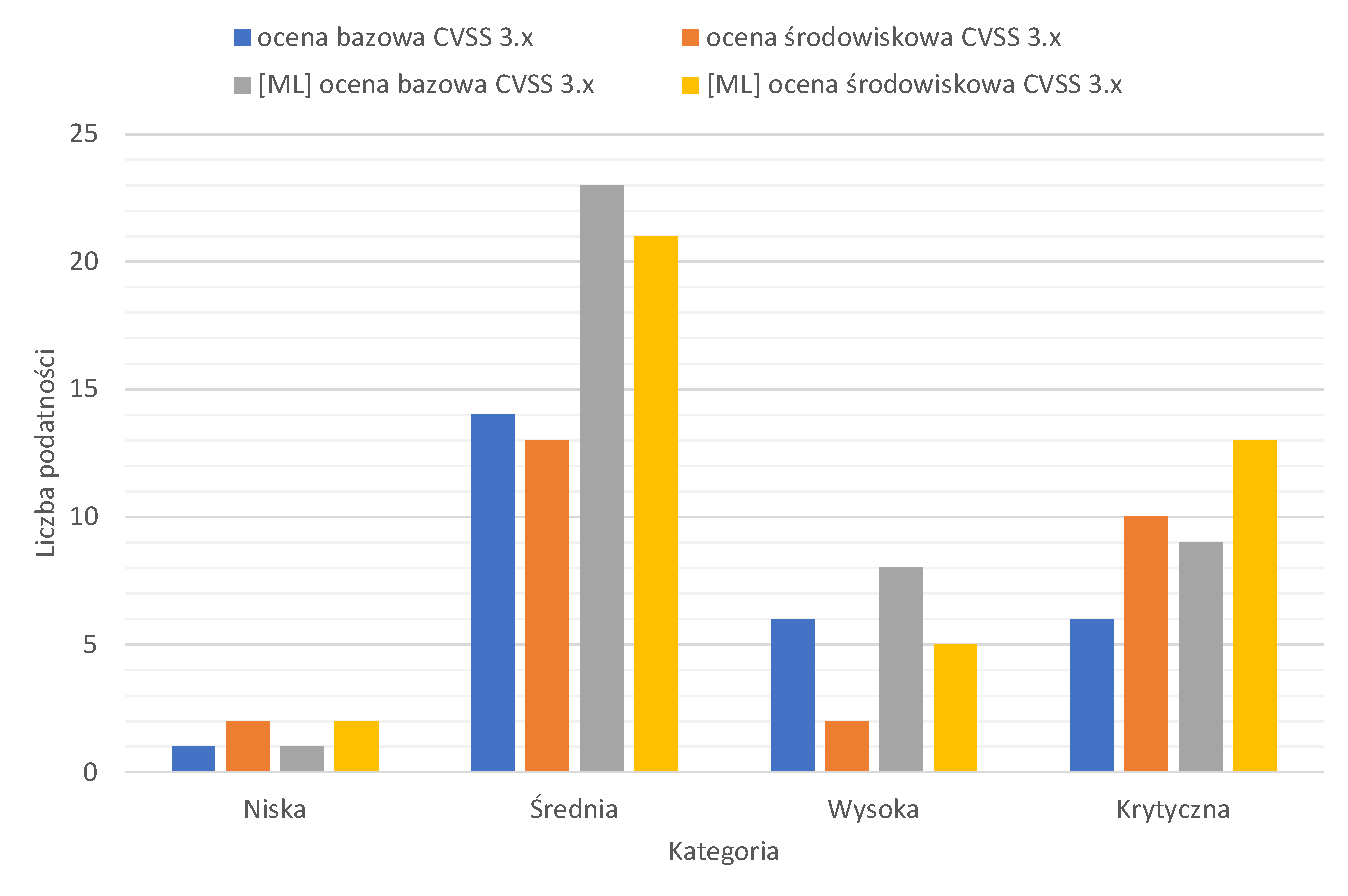
\includegraphics[width=.9\textwidth]{Chapters/Eksperymenty/env_A_results/cvss_3_ml.pdf}
\caption{Liczba wykrytych podatności dla każdej kategorii krytyczności według oceny bazowej i środowiskowej CVSS 3.x dla środowiska teleinformatycznego A.}
\label{fig:chapter6:env_a:cvss_3}
\end{figure}


\bigbreak
Rysunek \ref{fig:chapter6:env_a:cvss_3_changes_ml} przedstawia liczbę wszystkich podatności zmodyfikowanych dla danej wartości różnicy pomiędzy oceną bazową a środowiskową CVSS 3.x w przypadku środowiska teleinformatycznego A. Wyniki przedstawione na rysunku \ref{fig:chapter6:env_a:cvss_3_changes_ml} dotyczą rozpatrywanego przypadku pierwszego, w którym to uwzględnione są podatności z obliczoną oceną bazową CVSS 3.x za pomocą uczenia maszynowego. Parametry środowiskowe $CIA$ dla 5 wskazanych zasobów spowodowały modyfikację 19 ocen bazowych w zakresie od -2.1 do 1.9, co stanowi 46.3\% wszystkich wykrytych podatności. Pozostałe 22 podatności zostały wykryte na zasobach, dla których administrator środowiska A nie dostarczył żadnych informacji. 

\begin{figure}[!ht]
\centering
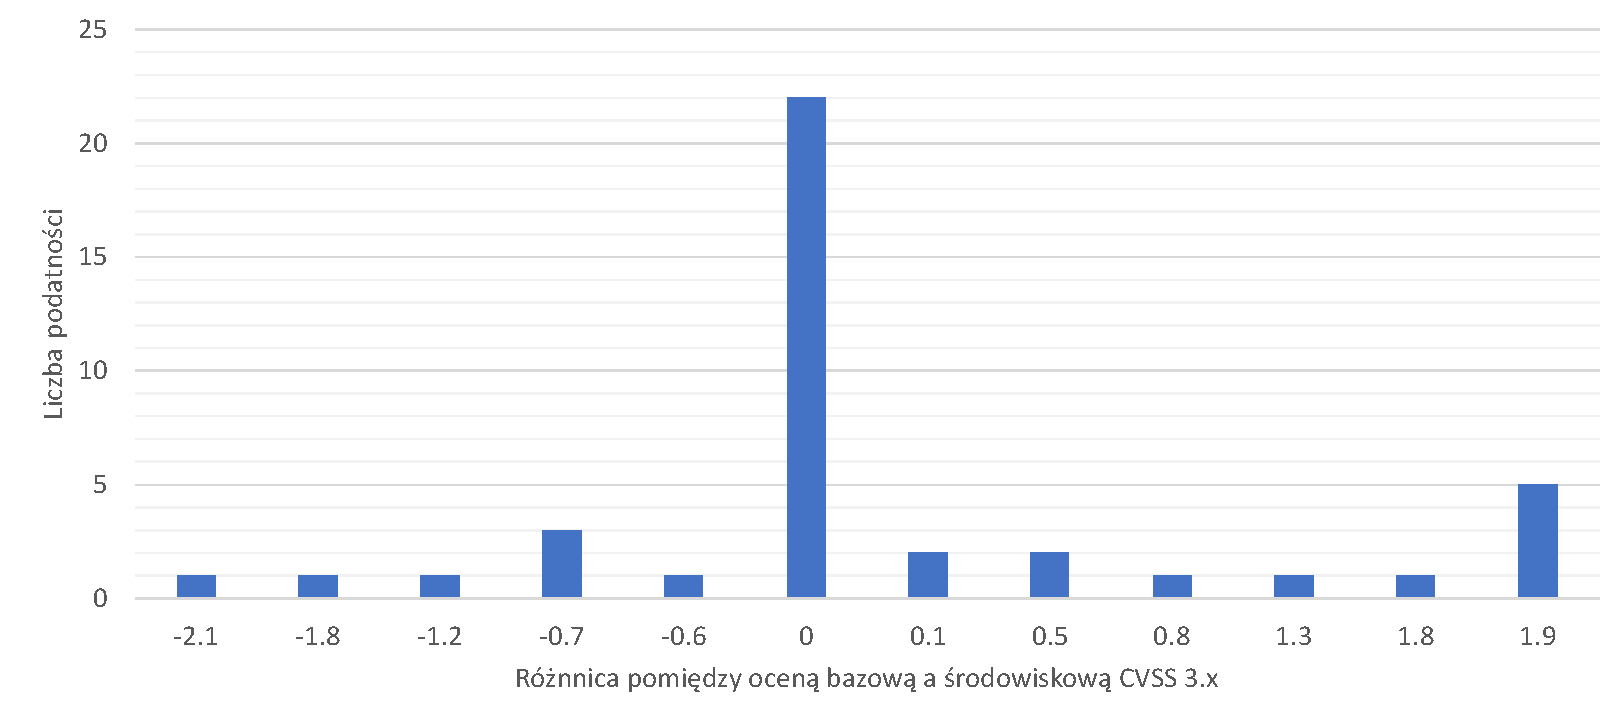
\includegraphics[width=.9\textwidth]{Chapters/Eksperymenty/env_A_results/changes_cvss_3_ml.pdf}
\caption{Liczba wszystkich podatności zmodyfikowanych dla danej wartości różnicy pomiędzy oceną bazową a środowiskową CVSS 3.x w przypadku środowiska teleinformatycznego A.}
\label{fig:chapter6:env_a:cvss_3_changes_ml}
\end{figure}

\bigbreak
Rysunek \ref{fig:chapter6:env_a:cvss_3_changes} przedstawia liczbę podatności zmodyfikowanych dla danej wartości różnicy pomiędzy oceną bazową a środowiskową CVSS 3.x w przypadku środowiska teleinformatycznego A. Wyniki przedstawione na rysunku \ref{fig:chapter6:env_a:cvss_3_changes} dotyczą rozpatrywanego przypadku drugiego, w którym to pomijane są podatności nie posiadające oceny bazowej CVSS 3.x. Parametry środowiskowe $CIA$ dla 5 wskazanych zasobów spowodowały modyfikacje 14 ocen bazowych w zakresie od -1.8 do 1.9, co stanowi 31.7\% wszystkich wykrytych podatności. Wyniki przedstawiające liczbę podatności zmodyfikowanych dla obu rozpatrywanych przypadków pozwalają na stwierdzenie, że każda informacja na temat środowiska może wpłynąć na zmianę w klasyfikacjach krytyczności podatności. Dodatkowo zmiana w klasyfikacjach krytyczności podatności wpływa na priorytetyzacje napraw podatności. Wykorzystanie mechanizmu konwersji oceny bazowej CVSS 2.0 do 3.x za pomocą uczenia maszynowego pozwala na uwzględnienie wszystkich wykrytych podatności w procesie zarządzania podatnościami dla analizowanego środowiska teleinformatycznego A.

\begin{figure}[!ht]
\centering
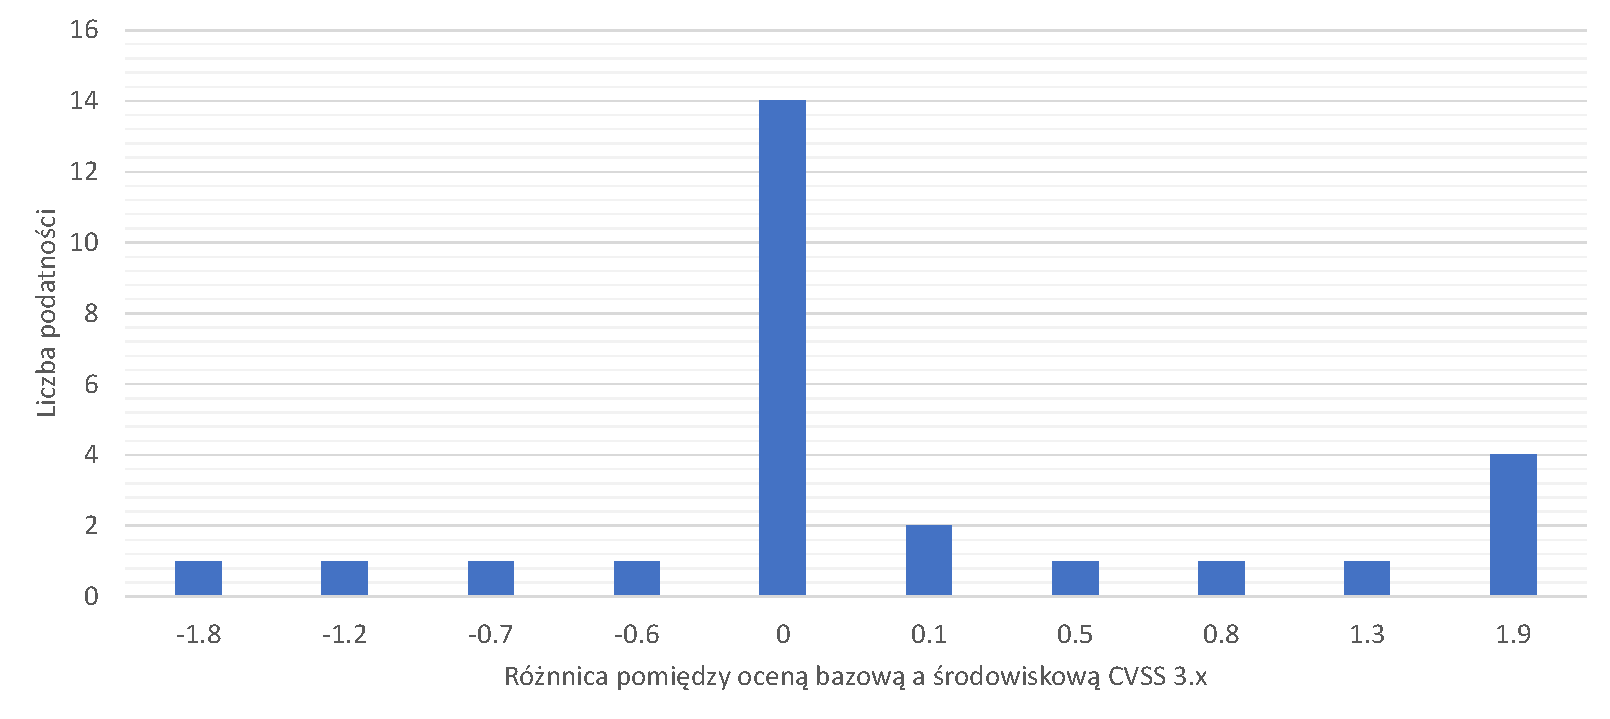
\includegraphics[width=.9\textwidth]{Chapters/Eksperymenty/env_A_results/changes_cvss_3.pdf}
\caption{Liczba podatności zmodyfikowanych dla danej wartości różnicy pomiędzy oceną bazową a środowiskową CVSS 3.x w przypadku środowiska teleinformatycznego A.}
\label{fig:chapter6:env_a:cvss_3_changes}
\end{figure}

\bigbreak
Tabela \ref{tab:chapter6:env_a:changes_ml} przedstawia liczbę zmian w kategoriach krytyczności podatności dla środowiska teleinformatycznego A po uwzględnieniu parametrów środowiskowych $CIA$ przy wykorzystaniu metod konwersji oceny bazowej CVSS 2.0 do 3.x za pomocą uczenia maszynowego. Największa zmiana w liczbie podatności została odnotowana dla kategorii krytycznej (+4) oraz wysokiej (-3). Dla zasobów posiadających wartości parametrów środowiskowych $CIA$ wykryto 29 podatności, co stanowi 70.71\% wszystkich podatności, 65.5\% z nich zmieniło swoją kategorię. W ogólnym ujęciu 24.39\% podatności zmieniło swoją kategorię z powodu wpływu wartości parametrów środowiskowych $CIA$ dla 5 zasobów. Uzyskane wyniki pozwalają na wyciągnięcie dwóch wniosków. Pierwszy mówi o tym, że możliwe jest wykorzystanie mechanizmu konwersji oceny bazowej CVSS 2.0 do 3.x do pełnej implementacji modelu zarządzania podatnościami opartego na ocenie środowiskowej CVSS 3.x dla wszystkich podatności. Natomiast drugi wniosek pozwala na stwierdzenie, że każda dodatkowa informacja na temat monitorowanego środowiska wpływa na priorytetyzacje napraw podatności poprzez możliwość zmiany kategorii krytyczności podatności.


\begin{table}[tbh]
\caption{Liczba zmian w kategoriach podatności dla środowiska teleinformatycznego A z wykorzystaniem metod konwersji oceny bazowej CVSS 2.0 do CVSS 3.x za pomocą uczenia maszynowego.}
\begin{center}
\label{tab:chapter6:env_a:changes_ml}
\begin{tabular}{cccc}
\hline \noalign {\smallskip}
\textbf{Kategoria}  & \textbf{[ML] ocena bazowa} & \textbf{[ML] ocena środowiskowa} & \textbf{Różnica} \\
                      & \textbf{CVSS 3.x} & \textbf{CVSS 3.x} & \\
  \hline
  Niska         &      1 &      2  &  +1          \\
                &        &         &  (+100\%)     \\
  Średnia       &     23 &      21 &  -2           \\
                &        &         &  (-8.69\%)       \\
  Wysoka        &      8 &       5 &  -3           \\
                &        &         &  (-37.5\%)   \\
  Krytyczna     &      9 &      13 &  +4          \\
                &        &         &  (+44.44\%)   \\
\hline \noalign {\smallskip}
\textbf{Razem}  &     41 &       41& 10 \\
                &        &         & (24.39\%) \\
\hline \noalign {\smallskip}
\end{tabular}
\end{center}
\end{table}

\bigbreak
Tabela \ref{tab:chapter6:env_a:changes} przedstawia liczbę zmian w kategoriach krytyczności podatności po uwzględnieniu parametrów środowiskowych $CIA$ dla środowiska teleinformatycznego A. Wyniki przedstawione w tabeli \ref{tab:chapter6:env_a:changes} nie uwzględniają mechanizmu konwersji oceny bazowej CVSS 2.0 do 3.x za pomocą uczenia maszynowego, to znaczy, że nie obejmują podatności, które nie posiadają oceny bazowej CVSS 3.x. Największa zmiana w liczbie podatności została odnotowana dla kategorii krytycznej (+4) oraz wysokiej (-4). Dla zasobów posiadających wartości parametrów środowiskowych $CIA$ wykryto 22 podatności, co stanowi 53.7\% wszystkich podatności, 59.1\% z nich zmieniło swoją kategorię. W ogólnym ujęciu 37\% podatności zmieniło swoją kategorię z powodu wpływu wartości parametrów środowiskowych $CIA$ dla 5 zasobów. Pomimo nieuwzględnienia wszystkich wykrytych podatności, parametry środowiskowe $CIA$ spowodowały znaczą zmianę w kategoriach krytyczności. Uzyskane wyniki pozwalają na wyciągnięcie wniosku mówiącego o tym, że znajomość parametrów środowiskowych $CIA$ tylko dla części monitorowanych zasobów pozwala na lepsze dopasowanie podatności, nawet w przypadku, gdy administrator akceptuje ryzyko, w którym pomija naprawę podatności nie posiadające ocenę bazową CVSS 3.x.

\begin{table}[tbh]
\caption{Liczba zmian w kategoriach podatności po uwzględnieniu parametrów środowiskowych $CIA$ dla środowiska teleinformatycznego A.}
\begin{center}
\label{tab:chapter6:env_a:changes}
\begin{tabular}{cccc}
\hline \noalign {\smallskip}
\textbf{Kategoria} & \textbf{ocena bazowa} & \textbf{ocena środowiskowa} & \textbf{Różnica} \\
                      & \textbf{CVSS 3.x} & \textbf{CVSS 3.x} & \\
  \hline
  Niska         &      1 &      2  &  +1          \\
                &        &         &  (+100\%)     \\
  Średnia       &     14 &      13 &  -1           \\
                &        &         &  (-7.1\%)       \\
  Wysoka        &      6 &       2 &  -4           \\
                &        &         &  (-66.7\%)   \\
  Krytyczna     &      6 &      10 &  +4          \\
                &        &         &  (+66.7\%)   \\
\hline \noalign {\smallskip}
\textbf{Razem}  &     27 &      27 & 10 \\
                &        &         & (37\%) \\
\hline \noalign {\smallskip}
\end{tabular}
\end{center}
\end{table}

\bigbreak
Tabela \ref{tab:chapter6:env_a:time_results_cvss_3} przedstawia liczbę roboczogodzin wymaganą do usunięcia istotnych podatności bezpieczeństwa dla środowiska teleinformatycznego A. W przypadku ocen bazowych CVSS 3.x szacunkowa liczba roboczogodzin została obliczona za pomocą wzorów: $T_{Base3}$ - \ref{eq:cvss3}, $T_{Base3'}$ - \ref{eq:cvss2prim}. W przypadku oceny środowiskowej CVSS 3.x szacunkowa liczba roboczogodzin została obliczona za pomocą wzoru \ref{eq:cvss3e}. Wartości dla czasów $T_{Base3}$ obliczone zostały przy założeniu, że administrator musi naprawić tylko podatności o kategorii krytycznej, wysokiej i średniej, w związku z czym akceptuje ryzyko związane z istnieniem w systemie podatności o krytyczności niskiej. Ponadto należy zauważyć, że w przypadku priortetyzacji opartej na ocenie bazowej CVSS 3.x, która nie uwzględnia danych środowiskowych wśród podatności sklasyfikowanych jako podatności o krytyczności niskiej, mogą się znajdować podatności o wyższej krytyczności, na przykład wysokiej. Wartości czasów $T_{Base3'}$ obliczone zostały zatem przy założeniu, że w celu zapewnienia bezpieczeństwa systemu administrator musi naprawić wszystkie podatności, ponieważ (jak opisano szczegółowo w rozdziale \ref{sec:wplyw_cvss3}) nie ma pewności, czy podatność z otrzymaną oceną bazową CVSS 3.x zachowa tę ocenę po uwzględnieniu danych środowiskowych. Natomiast wartości dla czasów $T_{Env3}$ obliczone zostały przy założeniu, że wszystkie oceny podatności zostały sklasyfikowane dokładnie (Rozdział \ref{sec:modele-zarzadzaia-podatnosciami}). Gdy porówna się szacowane liczby roboczogodzin otrzymane dla $T_{Base3}$ z $T_{Base3'}$, można zauważyć wzrost szacowanej liczy roboczogodzin dla wszystkich rozpatrywanych przypadków ($T_{FIX_{MIN}}$, $T_{FIX_{AVERAGE}}$, $T_{FIX_{MAX}}$), który wynosi 3.7\%. Ponadto można zaobserwować, że naprawienie wszystkich podatności według otrzymanej priorytetyzacji za pomocą oceny bazowej CVSS 3.x redukuje ryzyko nienaprawienia podatności niedoszacowanej z 34.1\% do 31.7\%. Gdy porówna się otrzymane wyniki dla $T_{Base3}$ i $T_{Env3}$, można zauważyć, że średni zysk w postaci obniżenia szacowanej liczby roboczogodzin dla wszystkich rozpatrywanych przypadków wynosi 3.8\%. Wykorzystanie priorytetyzacji za pomocą oceny środowiskowej CVSS 3.x obniża ryzyko z związane z nienaprawieniem podatności niedoszacowanej z 34.1\% do 29.1\%. Natomiast gdy porówna się wyniki otrzymane dla $T_{Base3'}$ i $T_{Env3}$, można zauważyć średni zysk w postaci obniżenia szacowanej liczby roboczogodzin dla wszystkich rozpatrywanych przypadków wynoszący 7\%. Ponadto wykonanie napraw podatności za pomocą prioretetyzacji podatności według oceny środowiskowej CVSS 3.x powoduje utrzymanie ryzyka dotyczącego wykorzystania nienaprawionej podatności przez atakującego na poziomie 29.1\%. W przypadku wykorzystania metod konwersji CVSS 2.0 do CVSS 3.x za pomocą uczenia maszynowego otrzymane wyniki dla $T_{Base3}$ i $T_{Base3ML}$ przedstawiają wzrost szacowanej liczby roboczogodzin o 51\%. Dodatkowo wykorzystanie metod konwersji oceny bazowej CVSS 2.0 do 3.x powoduje redukcję ryzyka dotyczącego możliwości wykorzystania podatności nienaprawionej przez atakującego z 34.1\% do 2.4\%. Natomiast gdy porówna się otrzymane wyniki dla $T_{Base3}$ i $T_{Env3ML}$, możemy zauważyć wzrost szacowanej liczby roboczogodzin o 47.6\%. Dodatkowo wykonanie pioretetyzacji napraw podatności za pomocą oceny środowiskowej CVSS 3.x z wykorzystaniem metod konwersji oceny bazowej CVSS 3.x redukuje ryzyko dotyczące nienaprawienia podatności, która może zostać wykorzystana przez atakującego, z 34.1\% do 2.4\%.

\begin{table}[tbh]
\caption{Liczba roboczogodzin wymagana do usunięcia istotnych podatności bezpieczeństwa dla środowiska teleinformatycznego A. W przypadku ocen bazowych CVSS 3.x szacunkowa liczba roboczogodzin została obliczona za pomocą wzorów: $T_{Base3}$ - \ref{eq:cvss3}, $T_{Base3'}$ - \ref{eq:cvss2prim}. W przypadku oceny środowiskowej CVSS 3.x szacunkowa liczba roboczogodzin została obliczona za pomocą wzoru \ref{eq:cvss3e}.}
\begin{center}
\label{tab:chapter6:env_a:time_results_cvss_3}
\begin{tabular}{c|ccc|c}
\hline
                 & \textbf{$T_{FIX_{MIN}}$} & \textbf{$T_{FIX_{AVERAGE}}$} & \textbf{$T_{FIX_{MAX}}$ }  & Średnia \% zmiana \\
\hline
$T_{Base3}$      &                         29h &              120h &    237h         &        \\
$T_{Base3'}$     &                         30h &            124.5h &    246h         &         \\
Różnica          &                +1h (+3.4\%) &    +4.5h (+3.7\%) &  +9h (+3.8\%) & +3.7\%   \\  
\hline
$T_{Base3}$      &                         29h &            120h &      237h         &        \\
$T_{Env3}$       &                         28h &            115.5h &    228h         &         \\
Różnica          &                -1h (-3.4\%) &    -4.5h (-3.8\%) &  -9h (-3.8\%) & -3.8\%   \\  
\hline
$T_{Base3'}$     &                         30h &            124.5h &    246h         &        \\
$T_{Env3}$       &                         28h &            115.5h &    228h         &         \\
Różnica          &                -2h (-6.6\%) &    -9h (-7.2\%) &  -18h (-7.3\%) & -7\%   \\  
\hline
$T_{Base3}$    &                      29h &            120h &    237h         &         \\
$T_{Base3ML}$&                        43h &          183h &      363h         &         \\
Różnica          &              +14h (+48\%) & +63h (+52\%) & +126h (+53\%) & +51\% \\  
\hline
$T_{Base3}$  &                             29h &            120h &    237h        &         \\
$T_{Env3ML}$     &                         42h &          178.5h &    354h        &         \\
Różnica          &               +13h (+44.8\%)  &  +58.5h (+48.5\%) & +117h (+49.3\%) & +47.6\% \\  
\hline
$T_{Base3ML}$    &                         43h &            183h &    363h         &         \\
$T_{Env3ML}$     &                         42h &          178.5h &    354h        &         \\
Różnica          &               -1h (-2.3\%)  &  -4.5h (-2.6\%) & -9h (-2.5\%) & -2.4\% \\  
\hline
\end{tabular}
\end{center}
\end{table}

\bigbreak
Jak wykazano w przeprowadzonej analizie, parametry środowiskowe $CIA$ mają znaczący wpływ na priorytetyzacje podatności bezpieczeństwa infrastruktury informatycznej, pomimo posiadania parametrów środowiskowych $CIA$ tylko dla 5 skanowanych zasobów. Parametry środowiskowe $CIA$ mają wpływ na szacowaną liczbę roboczogodzin wymaganą do usunięcia istotnych podatności bezpieczeństwa środowiska teleinformatycznego A w procesie zarządzania podatnościami (Rozdział \ref{sec:proces-zarzadzania-podatnosciami}). Wykorzystanie modelu zarządzania podatnościami opartego na ocenie środowiskowej CVSS 3.x (Rysunek \ref{fig:chapter1:vm-model-cvss3e}) z metodami konwersji oceny bazowej CVSS 2.0 do 3.x pozwala na lepsze dopasowanie kategorii podatności, a tym samym wpływa na priorytetyzacje napraw podatności dla otrzymanych danych, opisanych w rozdziale \ref{sec:desc_a}. Jak wynika z przeprowadzonej analizy, możliwe jest otrzymanie wyników oceny środowiskowej niezwłocznie po zakończonym procesie skanowania, co w rezultacie daje zysk w postaci obniżenia szacowanej liczby roboczogodzin o 7\%, oraz redukcje ryzyka nienaprawionych podatności niedoszacowanych z 34.1\% do 29.1\%. W przypadku wykorzystania metod konwersji CVSS 2.0 do CVSS 3.x możliwa jest redukcja ryzyka nienaprawienia podatności niedoszacowanych z 34.1\% do 2.4\%, jednocześnie obniżając szacowaną liczbę roboczogodzin potrzebnych do naprawienia wszystkich podatności o 2.4\%.

%%%%%%%%%%%%%%%%%%%%%%%%%%%%%%%%%%%%%%%%%%%%%%%%

%%%%%%%%%%%%%%%%%%%%%%%%%%%%%%%%%%%%%%%%%%%%%%%%

\subsubsection{Podsumowanie wyników analizy dla środowiska A}
Na podstawie wyników przedstawionych w podrozdziale ''Analiza wpływu parametrów środowiskowych na ocenę bazową CVSS 2.0'' można stwierdzić, że dla oceny środowiskowej wszystkie podatności zostały przydzielone do kategorii niskiej. Wpływ na to ma parametr $TD$, który osiągnął maksymalną wartość 13\%. Dodatkowo z analizy otrzymanych wyników można stwierdzić, że dodanie do oceny bazowej CVSS 2.0 danych środowiskowych powoduje znaczącą redukcję szacowanej liczby roboczogodzin wymaganą do usunięcia istotnych podatności wykrytych w środowisku teleinformatycznym A. Gdy porównamy wyniki otrzymane dla oceny bazowej CVSS 2.0 ($T_{Base2}$) z oceną środowiskową CVSS 2.0 ($T_{Env2}$), można zauważyć, że średni zysk w postaci obniżenia szacowanej liczby roboczogodzin wynosi 95.8\%. Wykorzystanie priorytetyzacji za pomocą oceny środowiskowej CVSS 2.0 pozwala na obniżenie ryzyka związanego z nienaprawieniem podatności niedoszacowanej z 10\% do 0\%. Wyniki przedstawione w podrozdziale ''Analiza wpływu parametrów środowiskowych na ocenę bazową CVSS 2.0'' potwierdzają wadę oceny środowiskowej CVSS 2.0 polegającą na tym, że parametr $TD$, który służy do ustalania liczby systemów wrażliwych na daną podatność, znacząco zaniża oceny wszystkich podatności. Dlatego konieczne było rozważenie modelu zarządzania podatnościami, który opiera się na standardzie CVSS 3.x.

\bigbreak
Na podstawie wyników przedstawionych w podrozdziale ''Analiza wpływu parametrów środowiskowych na ocenę bazową CVSS 3.x'' można stwierdzić, że wykorzystany mechanizm uczenia maszynowego wykonał obliczenia dla 34\% podatności wykrytych w środowisku teleinformatycznym A, które nie posiadają oceny bazowej CVSS 3.x z błędem klasyfikacji kategorii krytyczności wynoszącym 14\%, co oznacza, że można oczekiwać 2 podatności błędnie sklasyfikowanych, pozwalając tym samym na pełną implementację modelu zarządzania podatnościami opartego na standardzie CVSS 3.x (Rysunek \ref{fig:chapter1:vm-model-cvss3}, \ref{fig:chapter1:vm-model-cvss3e}). Z analizy otrzymanych wyników można także stwierdzić, że wpływ parametrów środowiskowych $CIA$ spowodował zmianę kategorii krytyczności dla 24.39\% podatności, co ma bezpośredni przekład na szacowaną liczbę roboczogodzin potrzebną do usunięcia istotnych podatności wykrytych w środowisku teleinformatycznym A. Gdy porównamy wyniki otrzymane dla oceny bazowej CVSS 3.x bez zastosowania metod konwersji oceny bazowej CVSS 2.0 do 3.x ($T_{Base3}$) z oceną środowiskową CVSS 3.x z zastosowaniem metod konwersji oceny bazowej CVSS 2.0 do 3.x. ($T_{Env3ML}$), można zauważyć wzrost szacowanej liczby roboczogodzin o 47.6\%. Wzrost szacowanej liczby roboczogodzin wynika z uwzględnienia wszystkich podatności po zastosowaniu metod konwersji oceny bazowej CVSS 2.0 do 3.x za pomocą uczenia maszynowego. Natomiast wykonanie priorytetyzacji napraw podatności za pomocą oceny środowiskowej CVSS 3.x z wykorzystaniem metod konwersji oceny bazowej CVSS 2.0 do 3.x redukuje ryzyko dotyczące nienaprawienia podatności, która może zostać wykorzystana przez atakującego, z 34.1\% do 2.4\%.

%%%%%%%%%%%%%%%%%%%%%%%%%%%%%%%%%%%%%%%%%%%%%%%%

%%%%%%%%%%%%%%%%%%%%%%%%%%%%%%%%%%%%%%%%%%%%%%%%
\subsection{Analiza dla środowiska teleinformatycznego B}


%%%%%%%%%%%%%%%%%%%%%%%%%%%%%%%%%%%%%%%%%%%%%%%%

%%%%%%%%%%%%%%%%%%%%%%%%%%%%%%%%%%%%%%%%%%%%%%%%
\subsubsection{Analiza wpływu parametrów środowiskowych na ocenę bazową CVSS 2.0}

Rysunek \ref{fig:chapter6:env_b:cvss_2} przedstawia liczbę wykrytych podatności dla każdej kategorii krytyczności według oceny bazowej i środowiskowej CVSS 2.0. Na podstawie wyników pokazanych na rysunku \ref{fig:chapter6:env_b:cvss_2} można stwierdzić, że dla oceny środowiskowej CVSS 2.0 znaczna większość podatności została przydzielona do kategorii niskiej. Wpływ na to ma parametr $TD$ (Rozdział \ref{sec:td}), który osiągnął maksymalną wartość 25\%, co zostało przedstawione na rysunku \ref{fig:chapter6:env_b:cvss_2_td}. Parametr $TD$ wskazuje procent zasobów wrażliwych na konkretną podatność. Rysunek \ref{fig:chapter6:env_b:cvss_2_td} przedstawia wartość parametru $TD$ dla wykrytych podatności w środowisku teleinformatycznym A. Wpływ pozostałych parametrów środowiskowych na kategorię krytyczności podatności, $CDP$ (Rozdział \ref{sec:cdp}) oraz $CIA$ (Rozdział \ref{sec:cia_desc}) jest niezauważalny, ponieważ parametr $TD$ osiąga maksymalną wartość 25\%. Wyniki przedstawione na rysunku \ref{fig:chapter6:env_b:cvss_2} potwierdzają, że model zarządzania podatnościami, który wykorzystuje ocenę środowiskową CVSS 2.0, ma istotną wadę. Wada ta polega na tym, że parametr $TD$, który służy do ustalania liczby systemów wrażliwych na daną podatność, znacząco zaniża oceny wszystkich podatności. Dlatego też model zarządzania podatnościami oparty o ocenę środowiskową CVSS 2.0, nie jest dokładną miarą bezpieczeństwa infrastruktury teleinformatycznej. Konieczne jest zatem rozważenie modelu zarządzania podatnościami, który opiera się na standardzie CVSS 3.x. Niemniej jednak należy zauważyć, że ocena środowiskowa CVSS 2.0 dostarcza bardzo ważnej informacji dla administratora. Mianowicie jeśli wartość parametru $TD$ jest niska, to w badanym środowisku teleinformatycznym wykryta podatność może zagrozić jedynie niewielkiej liczbie serwerów. Na przykład w środowisku C wykryto podatności, których wykorzystanie możne zagrozić co najwyżej 9 serwerom, tj. 25\% skanowanych zasobów.

\begin{figure}[!ht]
\centering
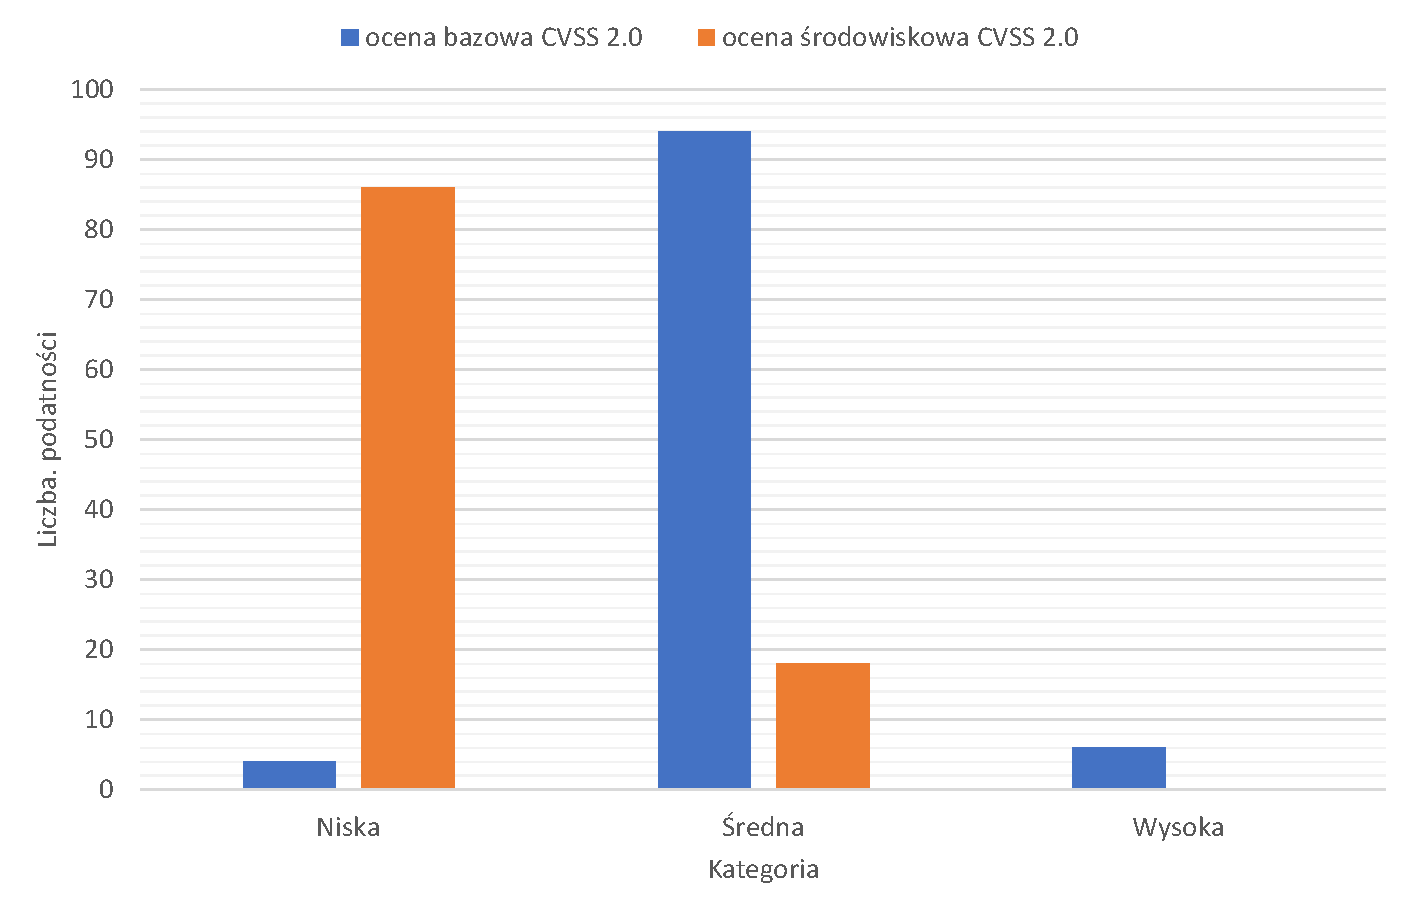
\includegraphics[width=.9\textwidth]{Chapters/Eksperymenty/env_B_results/cvss_2.pdf}
\caption{Liczba wykrytych podatności dla każdej kategorii krytyczności według oceny bazowej i środowiskowej CVSS 2.0 dla środowiska teleinformatycznego B.}
\label{fig:chapter6:env_b:cvss_2}
\end{figure}

\begin{figure}[!ht]
\centering
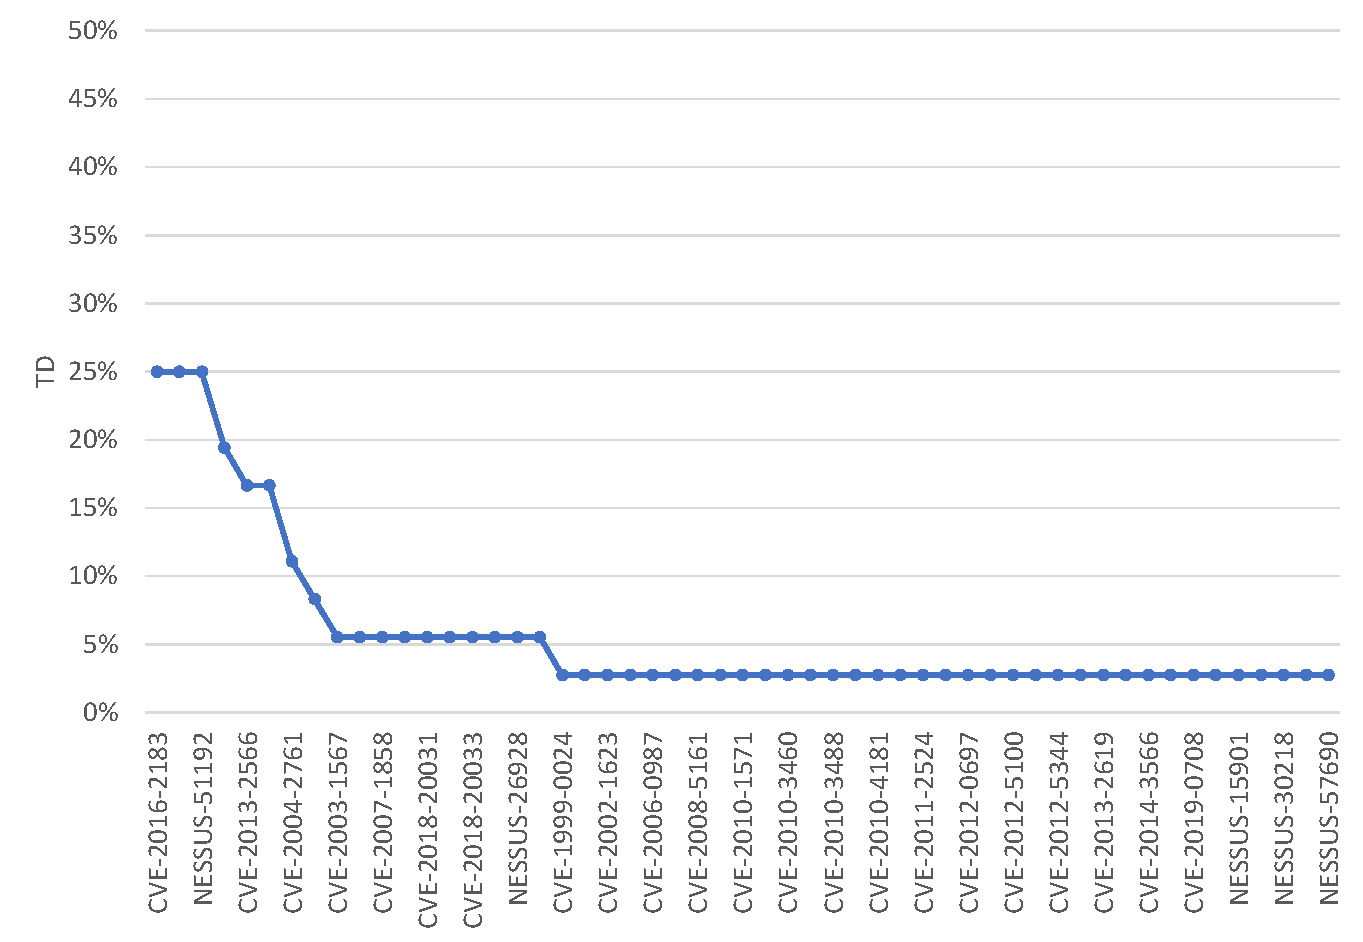
\includegraphics[width=.9\textwidth]{Chapters/Eksperymenty/env_B_results/cvss_2_td_env_b.pdf}
\caption{Wartość parametru $TD$ dla wykrytych podatności w środowisku teleinformatycznym B.}
\label{fig:chapter6:env_b:cvss_2_td}
\end{figure}

\bigbreak
Rysunek \ref{fig:chapter6:env_b:cvss_2_changes} przedstawia liczbę podatności zmodyfikowanych dla danej wartości różnicy pomiędzy oceną bazową a środowiskową CVSS 2.0 w przypadku środowiska teleinformatycznego B. Uwzględnienie parametrów środowiskowych $CIA$, $CDP$, $TD$ spowodowało zmianę wszystkich ocen bazowych CVSS 2.0 w przedziale od -7.5 do -1.2. Brak ocen bazowych niezmodyfikowanych spowodowany jest postacią równania \ref{eq:cvss2_es}, w którym to występuje mnożenie oceny końcowej przez wartość parametru środowiskowego $TD$ w celu otrzymania wartości oceny środowiskowej CVSS 2.0. Z liczby oraz zakresu zmian można wywnioskować, że w zbiorze wykrytych podatności znajdują się zagrożenia, które mogą mieć istotny wpływ na bezpieczeństwo monitorowanego środowiska. 

Zbiór wykrytych podatności w środowisku teleinformatycznym B składa się z dwóch podzbiorów: podatności posiadających obie oceny bazowe (CVSS 2.0 oraz CVSS 3.x) oraz podatności ze znaną jedynie oceną bazową w standardzie CVSS 2.0. W przypadku pierwszego podzbioru podatności posiadają ocenę bazową według standardu CVSS 3.x, w związku z czym priorytetyzacja naprawy zostanie ujęta w procesie zarządzania podatnościami za pomocą modelu \ref{fig:chapter1:vm-model-cvss3e} (Rozdział \ref{sec:proces-zarzadzania-podatnosciami}), ponieważ stosowanie oceny bazowej CVSS 3.x pozwala dokładniej ocenić krytyczność podatności, a zatem skuteczniej oszacować zagrożenia (Rozdział \ref{sec:modele-zarzadzaia-podatnosciami}). W przypadku drugiego podzbioru, który zawiera 50 (48\%) podatności, wykorzystano mechanizm konwersji oceny bazowej CVSS 2.0 do 3.x opisany w rozdziale \ref{sec:ml} w celu umożliwienia wykonania priorytetyzacji za pomocą modelu oceny środowiskowej CVSS 3.x (Rysunek \ref{fig:chapter1:vm-model-cvss3e}).

\begin{figure}[!ht]
\centering
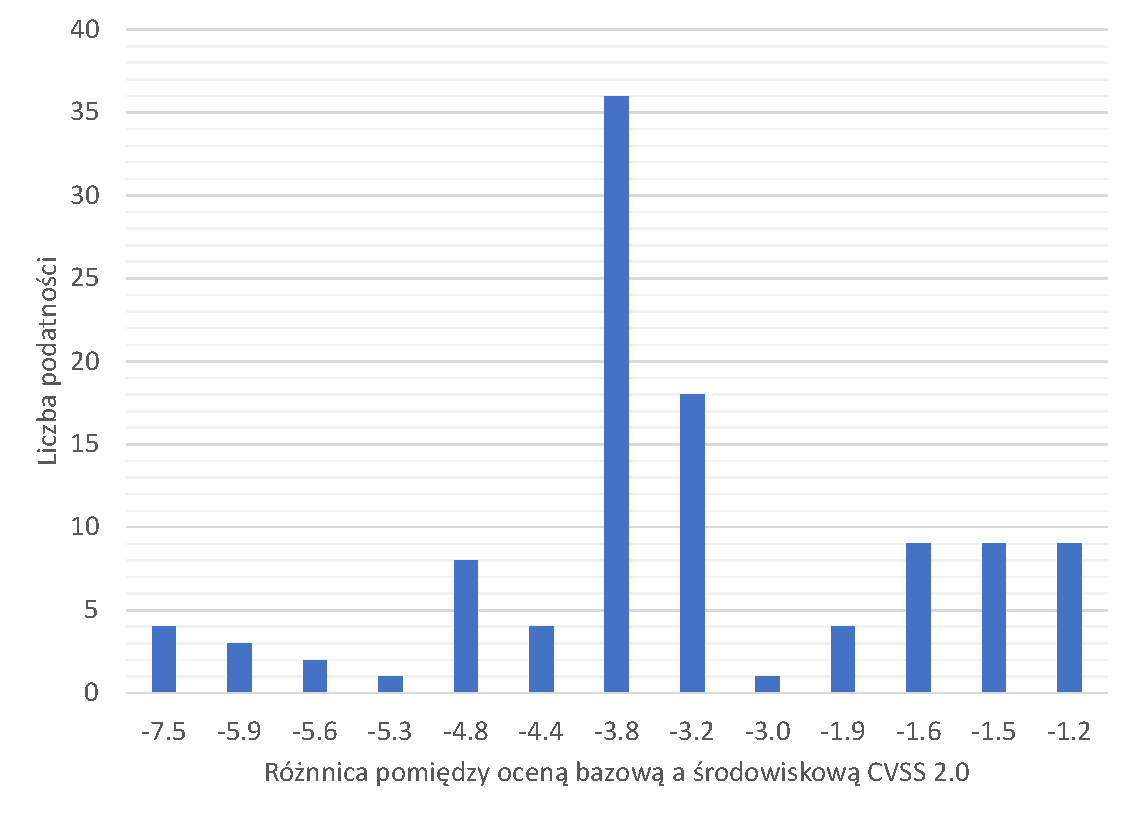
\includegraphics[width=.9\textwidth]{Chapters/Eksperymenty/env_B_results/changes_cvss_2.pdf}
\caption{Liczba podatności zmodyfikowanych dla danej wartości różnicy pomiędzy oceną bazową a środowiskową CVSS 2.0 w przypadku środowiska teleinformatycznego B.}
\label{fig:chapter6:env_b:cvss_2_changes}
\end{figure}

\bigbreak
Tabela \ref{tab:chapter6:env_b:time_results_cvss2} przedstawia liczbę roboczogodzin wymaganą do usunięcia istotnych podatności bezpieczeństwa dla środowiska teleinformatycznego B. W przypadku ocen bazowych CVSS 2.0 szacunkowa liczba roboczogodzin została obliczona za pomocą wzorów: $T_{Base2}$ - \ref{eq:cvss2}, $T_{Base2'}$ - \ref{eq:cvss2prim}. W przypadku oceny środowiskowej CVSS 2.0 szacunkowa liczba roboczogodzin została obliczona za pomocą wzoru \ref{eq:cvss2e}. Wartości dla czasów $T_{Base2}$ obliczone zostały przy założeniu, że administrator musi naprawić tylko podatności o krytyczności wysokiej i średniej, w związku z czym akceptuje ryzyko związane z istnieniem w systemie podatności o krytyczności niskiej. Ponadto należy zauważyć, że w przypadku priortetyzacji opartej na ocenie bazowej CVSS 2.0, która nie uwzględnia danych środowiskowych wśród podatności sklasyfikowanych jako podatności o krytyczności niskiej, mogą się znajdować podatności o wyższej krytyczności, na przykład wysokiej. Wartości czasów $T_{Base2'}$ obliczone zostały zatem przy założeniu, że w celu zapewnienia bezpieczeństwa systemu administrator musi naprawić wszystkie podatności, ponieważ (jak opisano szczegółowo w rozdziale \ref{sec:wplyw_cvss2}) nie ma pewności, czy podatność z otrzymaną oceną bazową CVSS 2.0 zachowa tę ocenę po uwzględnieniu danych środowiskowych. Natomiast wartości dla czasów $T_{Env2}$ obliczone zostały przy założeniu, że wszystkie oceny podatności zostały sklasyfikowane dokładnie (Rozdział \ref{sec:modele-zarzadzaia-podatnosciami}). Gdy porówna się szacowane liczby roboczogodzin otrzymane dla $T_{Base2}$ z $T_{Base2'}$, można zauważyć wzrost szacowanej liczby roboczogodzin dla wszystkich rozpatrywanych przypadków ($T_{FIX_{MIN}}$, $T_{FIX_{AVERAGE}}$, $T_{FIX_{MAX}}$), który wynosi 3.6\%. Ponadto można zaobserwować, że naprawienie wszystkich podatności według otrzymanej priorytetyzacji za pomocą oceny bazowej CVSS 2.0 redukuje ryzyko nienaprawienia podatności niedoszacowanej z 3.8\% do 0\%. Gdy porównamy otrzymane wyniki dla $T_{Base2}$ i $T_{Env2}$, można zauważyć, że średni zysk w postaci obniżenia szacowanej liczby roboczogodzin dla wszystkich rozpatrywanych przypadków wynosi 75\%. Wykorzystanie priorytetyzacji za pomocą oceny środowiskowej CVSS 2.0 pozwala na obniżenie ryzyka związanego z nienaprawieniem podatności niedoszacowanej z 3.8\% do 0\%. Natomiast gdy porówna się wyniki otrzymane dla $T_{Base2'}$ i $T_{Env2}$, można zauważyć, że średni zysk w postaci obniżenia szacowanej liczby roboczogodzin dla wszystkich rozpatrywanych przypadków wynosi 75.9\% i tym samym utrzymuje ryzyko związane z nienaprawieniem podatności niedoszacowanych na poziomie 0\%.

\begin{table}[tbh]
\caption{Liczba roboczogodzin wymagana do usunięcia podatności bezpieczeństwa dla środowiska teleinformatycznego B. W przypadku ocen bazowych CVSS 2.0 szacunkowa liczba roboczogodzin została obliczona za pomocą wzorów: $T_{Base2}$ - \ref{eq:cvss2}, $T_{Base2'}$ - \ref{eq:cvss2prim}. W przypadku oceny środowiskowej CVSS 2.0 szacunkowa liczba roboczogodzin została obliczona za pomocą wzoru \ref{eq:cvss2e}.}
\begin{center}
\label{tab:chapter6:env_b:time_results_cvss2}
\begin{tabular}{c|ccc|c}
\hline
                 & \textbf{$T_{FIX_{MIN}}$} & \textbf{$T_{FIX_{AVERAGE}}$} & \textbf{$T_{FIX_{MAX}}$ }  & Średnia \% zmiana \\
\hline
$T_{Base2}$      &                        119h &              469h &    919h         &        \\
$T_{Base2'}$     &                        123h &              486h &    955h         &         \\
Różnica          &                +4h (+3.4\%) &       +17h (+3.6\%) & +36h (+3.9\%) & +3.6\%   \\  
\hline
$T_{Base2}$      &                       119h &              469h &    919h         &         \\
$T_{Env2}$       &                        38h &            104.5h &    190h         &         \\
Różnica          &             -81h (-68\%) & -364.5h (-77.7\%) & -729h (-79.3\%) & -75\% \\  
\hline
$T_{Base2'}$     &                       123h &              486h &     955h        &         \\
$T_{Env2}$        &                       38h &            104.5h &     190h        &         \\
Różnica          &             -85h (-69.1\%) & -381.5h (-78.5\%) & -765h (-80.1\%) & -75.9\% \\  
\hline
\end{tabular}
\end{center}
\end{table}

\bigbreak
Jak wykazano w przeprowadzonej analizie, model zarządzania podatnościami, który wykorzystuje ocenę środowiskową CVSS 2.0, ma istotną wadę. Wada ta polega na tym, że parametr $TD$, który służy do ustalania liczby systemów wrażliwych na daną podatność, znacząco zaniża oceny wszystkich wykrytych podatności. W analizowanym środowisku teleinformatycznym B spowodował sklasyfikowanie znacznej większości podatności do kategorii niskiej. Dlatego też ocena środowiskowa CVSS 2.0 nie jest dokładną miarą bezpieczeństwa infrastruktury teleinformatycznej. Analiza wyników pozwala na wyciągnięcie kolejnego wniosku. Mianowicie model zarządzania podatnościami przy zastosowaniu oceny środowiskowej CVSS 2.0 (Rysunek \ref{fig:chapter1:vm-model-cvss2e}) może być wykorzystany do wykrywania podatności, które mogą zagrozić większej liczbie skanowanych zasobów. Taka informacja jest niezwykle cenna dla wszystkich osób zaangażowanych w proces zarządzania podatnościami (Rozdział \ref{sec:proces-zarzadzania-podatnosciami}), ponieważ pozwala na podjęcie szybkiej decyzji dotyczącej naprawy podatności oraz skrócenie czasu ich obecności w monitorowanej infrastrukturze teleinformatycznej.

%%%%%%%%%%%%%%%%%%%%%%%%%%%%%%%%%%%%%%%%%%%%%%%%

%%%%%%%%%%%%%%%%%%%%%%%%%%%%%%%%%%%%%%%%%%%%%%%%
\subsubsection{Analiza wpływu parametrów środowiskowych na ocenę bazową CVSS 3.x}

Rysunek \ref{fig:chapter6:env_b:cvss_3} przedstawia liczbę wykrytych podatności dla każdej kategorii krytyczności według oceny bazowej i środowiskowej CVSS 3.x dla środowiska teleinformatycznego B. Na podstawie wyników pokazanych na rysunku \ref{fig:chapter6:env_b:cvss_3} można stwierdzić, że dla oceny środowiskowej CVSS 3.x wszystkie podatności nie zmieniły kategorii krytyczności. Wpływ na to ma brak informacji od administratora środowiska teleinformatycznego B na temat parametrów środowiskowych $CIA$. W rezultacie bez dostarczonych informacji od administratora środowiska teleinformatycznego B, niemożliwe było wykonanie ponownej priorytetyzacji oraz oszacowanie zysków z wykorzystania modelu zarządzania podatnościami opartego o ocenę środowiskową CVSS 3.x (Rysunek \ref{eq:cvss2e}). Wyniki przedstawione na rysunkach \ref{fig:chapter6:env_a:cvss_3} oraz \ref{fig:chapter6:env_b:cvss_3} pokazują jak ważne jest posiadanie zbudowanej bazy inwentaryzacyjnej z określonymi wagami zasobów teleinformatycznych pod kątem wymagań ciągłości, integralności oraz dostępności w procesie zarządzania podatnościami.


\begin{figure}[!ht]
\centering
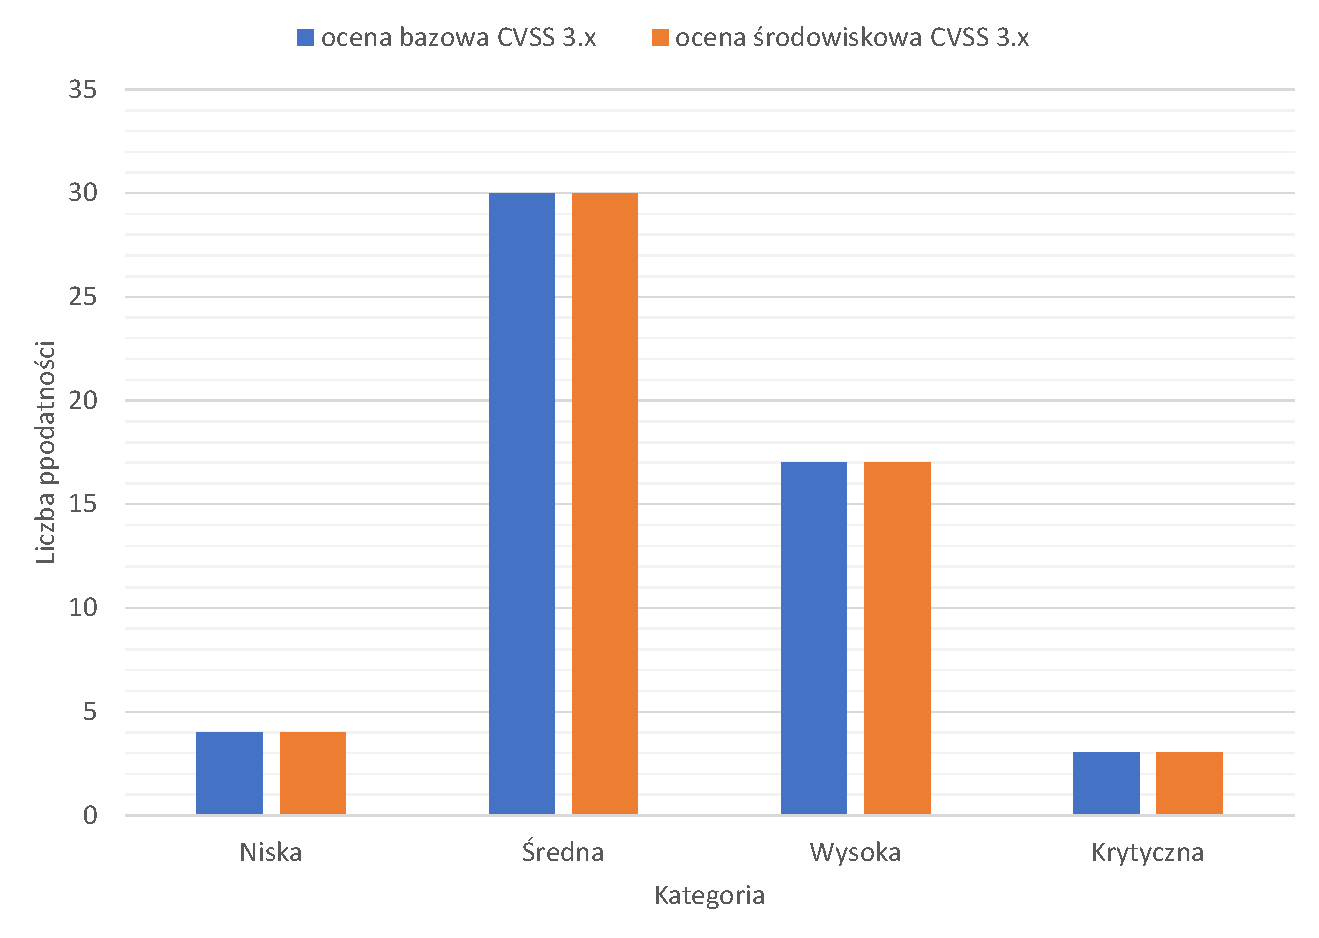
\includegraphics[width=.9\textwidth]{Chapters/Eksperymenty/env_B_results/cvss_3.pdf}
\caption{Liczba wykrytych podatności dla każdej kategorii krytyczności według oceny bazowej i środowiskowej CVSS 3.x dla środowiska teleinformatycznego B.}
\label{fig:chapter6:env_b:cvss_3}
\end{figure}

%%%%%%%%%%%%%%%%%%%%%%%%%%%%%%%%%%%%%%%%%%%%%%%%

%%%%%%%%%%%%%%%%%%%%%%%%%%%%%%%%%%%%%%%%%%%%%%%%

\subsubsection{Podsumowanie wyników analizy dla środowiska B}
Na podstawie wyników przedstawionych w podrozdziale ''Analiza wpływu parametrów środowiskowych na ocenę bazową CVSS 2.0' można stwierdzić, że dla oceny środowiskowej znacząca większość podatności zostały przydzielone do kategorii niskiej. Wpływ na to ma parametr $TD$, który osiągnął maksymalną wartość 25\%. Otrzymana maksymalna wartość oznacza, że w środowisku teleinformatycznym B wykryte zostały podatności, na które wrażliwe jest 9 skanowanych zasobów. Dlatego też wszystkie podatności, dla których parametr $TD$ ma wartość 25\%, zostały przydzielone do kategorii średniej. Dodatkowo z analizy otrzymanych wyników można stwierdzić, że dodanie do oceny bazowej CVSS 2.0 danych środowiskowych powoduje znaczącą redukcję szacowanej liczby roboczogodzin wymaganą do usunięcia istotnych podatności wykrytych w środowisku teleinformatycznym B. Gdy porównamy wyniki otrzymane dla oceny bazowej CVSS 2.0 ($T_{Base2}$) z oceną środowiskową CVSS 2.0 ($T_{Env2}$), można zauważyć, że średni zysk w postaci obniżenia szacowanej liczby roboczogodzin wynosi 75.9\%. Wykorzystanie priorytetyzacji za pomocą oceny środowiskowej CVSS 2.0 pozwala na obniżenie ryzyka związanego z nienaprawieniem podatności niedoszacowanej z 3.8\% do 0\%. Wyniki przedstawione w podrozdziale ''Analiza wpływu parametrów środowiskowych na ocenę bazową CVSS 2.0'' potwierdzają wadę oceny środowiskowej CVSS 2.0 polegającą na tym, że parametr $TD$, który służy do ustalania liczby systemów wrażliwych na daną podatność, znacząco zaniża oceny wszystkich podatności. Pomimo wspomnianej wady, na podstawie otrzymanych wyników, można dodatkowo stwierdzić, że wartość parametru $TD$ może być wykorzystana do wykrywania podatności, które mogą zagrozić większej liczbie skanowanych zasobów. Ponieważ jednak parametr $TD$ zaniża oceny wszystkich podatności, konieczne było rozważenie modelu zarządzania podatnościami, który opiera się na standardzie CVSS 3.x.

\bigbreak
Na podstawie wyników przedstawionych w podrozdziale ''Analiza wpływu parametrów środowiskowych na ocenę bazową CVSS 3.x'' można stwierdzić, że dla oceny środowiskowej CVSS 3.x wszystkie podatności nie zmieniły kategorii krytyczności. Wpływ na to ma brak dostarczonych informacji od administratora środowiska teleinformatycznego B na temat parametrów środowiskowych $CIA$. Z otrzymanych wyników można stwierdzić, że bez określonych parametrów środowiskowych $CIA$ niemożliwe jest wykonanie ponownej priorytetyzacji podatności dla modelu zarządzania podatnościami opartego o ocenę środowiskową CVSS 3.x (Rysunek \ref{fig:chapter1:vm-model-cvss3e}). W rezultacie na podstawie otrzymanych wyników można stwierdzić, że potwierdzają wniosek dotyczący istotności posiadania zbudowanej bazy zasobów, w której określone zostaną parametry $CIA$ dla każdego z monitorowanych zasobów.


%%%%%%%%%%%%%%%%%%%%%%%%%%%%%%%%%%%%%%%%%%%%%%%%

%%%%%%%%%%%%%%%%%%%%%%%%%%%%%%%%%%%%%%%%%%%%%%%%
\subsection{Analiza dla środowiska teleinformatycznego C}


%%%%%%%%%%%%%%%%%%%%%%%%%%%%%%%%%%%%%%%%%%%%%%%%

%%%%%%%%%%%%%%%%%%%%%%%%%%%%%%%%%%%%%%%%%%%%%%%%
\subsubsection{Analiza wpływu parametrów środowiskowych na ocenę bazową CVSS 2.0}
Rysunek \ref{fig:chapter6:env_c:cvss_2} przedstawia liczbę wykrytych podatności dla każdej kategorii krytyczności według oceny bazowej i środowiskowej CVSS 2.0. Na podstawie wyników pokazanych na rysunku \ref{fig:chapter6:env_c:cvss_2} można stwierdzić, że dla oceny środowiskowej CVSS 2.0 wszystkie podatności zostały przydzielone do kategorii niskiej. Wpływ na to ma parametr $TD$ (Rozdział \ref{sec:td}), który osiągnął maksymalną wartość 3\%, co zostało przedstawione na rysunku \ref{fig:chapter6:env_c:cvss_2_td}. Parametr $TD$ wskazuje procent zasobów wrażliwych na konkretną podatność. Rysunek \ref{fig:chapter6:env_c:cvss_2_td} przedstawia wartość parametru $TD$ dla wykrytych podatności w środowisku teleinformatycznym C. Wpływ pozostałych parametrów środowiskowych na kategorię krytyczności podatności, $CDP$ (Rozdział \ref{sec:cdp}) oraz $CIA$ (Rozdział \ref{sec:cia_desc}) jest niezauważalny, ponieważ parametr $TD$ osiąga maksymalną wartość 3\%. Wyniki przedstawione na rysunku \ref{fig:chapter6:env_c:cvss_2} potwierdzają, że model zarządzania podatnościami, który wykorzystuje ocenę środowiskową CVSS 2.0, ma istotną wadę. Wada ta polega na tym, że parametr $TD$, który służy do ustalania liczby systemów wrażliwych na daną podatność, znacząco zaniża oceny wszystkich podatności. Dlatego też model zarządzania podatnościami oparty o ocenę środowiskową CVSS 2.0 nie jest dokładną miarą bezpieczeństwa infrastruktury teleinformatycznej. Konieczne jest zatem rozważenie modelu zarządzania podatnościami, który opiera się na standardzie CVSS 3.x. Niemniej jednak należy zauważyć, że ocena środowiskowa CVSS 2.0 dostarcza bardzo ważnej informacji dla administratora. Mianowicie jeśli wartość parametru $TD$ jest niska, to w badanym środowisku teleinformatycznym wykryta podatność może zagrozić jedynie niewielkiej liczbie serwerów. Na przykład w środowisku C wykryto podatności, których wykorzystanie możne zagrozić co najwyżej 62 serwerom, tj. 3\% skanowanych zasobów.

\begin{figure}[!ht]
\centering
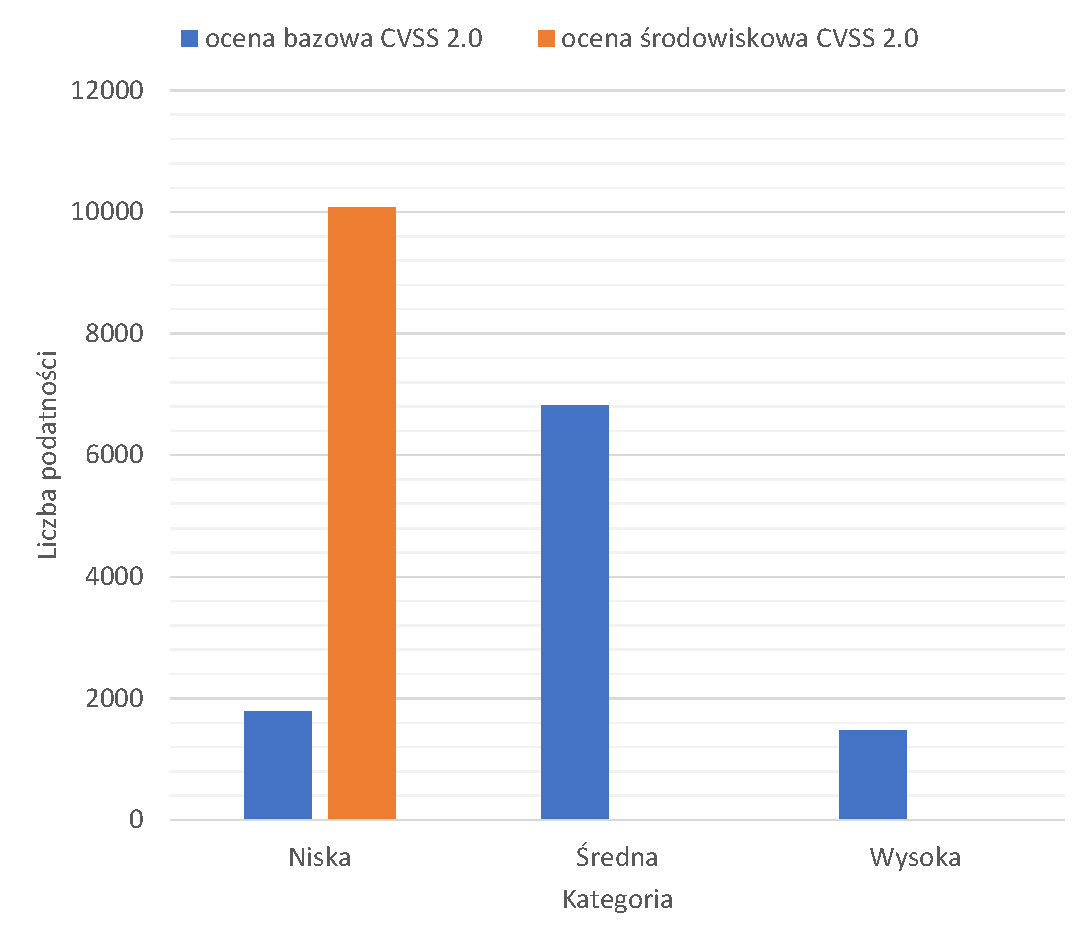
\includegraphics[width=.9\textwidth]{Chapters/Eksperymenty/env_C_results/cvss_2.pdf}
\caption{Liczba wykrytych podatności dla każdej kategorii krytyczności według oceny bazowej i środowiskowej CVSS 2.0 dla środowiska teleinformatycznego C.}
\label{fig:chapter6:env_c:cvss_2}
\end{figure}

\begin{figure}[!ht]
\centering
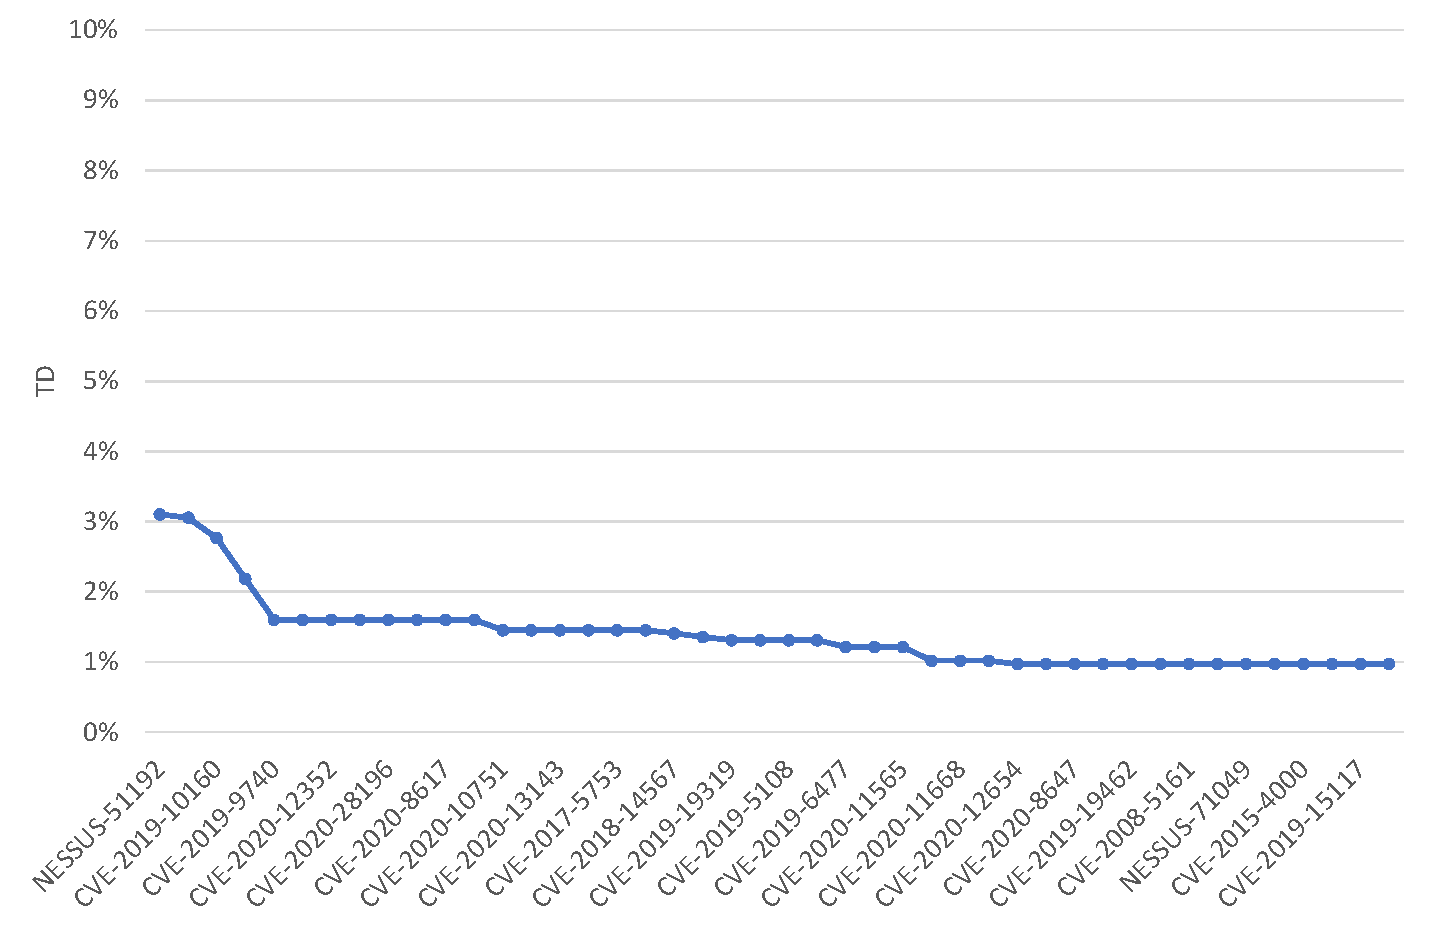
\includegraphics[width=.9\textwidth]{Chapters/Eksperymenty/env_C_results/cvss_2_td_env_c.pdf}
\caption{Wartość parametru $TD$ dla wykrytych podatności w środowisku teleinformatycznym C.}
\label{fig:chapter6:env_c:cvss_2_td}
\end{figure}

\bigbreak
Rysunek \ref{fig:chapter6:env_c:cvss_2_changes} przedstawia liczbę podatności zmodyfikowanych dla danej wartości różnicy pomiędzy oceną bazową a środowiskową CVSS 2.0 w przypadku środowiska teleinformatycznego C. Uwzględnienie parametrów środowiskowych $CIA$, $CDP$, $TD$ spowodowało zmianę wszystkich ocen bazowych CVSS 2.0 w przedziale od -10.0 do -1.2. Brak ocen bazowych niezmodyfikowanych spowodowany jest postacią równania \ref{eq:cvss2_es}, w którym to występuje mnożenie oceny końcowej przez wartość parametru środowiskowego $TD$ w celu otrzymania wartości oceny środowiskowej CVSS 2.0. Z liczby oraz zakresu zmian można wywnioskować, że w zbiorze wykrytych podatności znajdują się zagrożenia, które mogą mieć istotny wpływ na bezpieczeństwo monitorowanego środowiska. 

Zbiór wykrytych podatności w środowisku teleinformatycznym C składa się z dwóch podzbiorów: podatności posiadających obie oceny bazowe (CVSS 2.0 oraz CVSS 3.x) oraz podatności ze znaną jedynie oceną bazową w standardzie CVSS 2.0. W przypadku pierwszego podzbioru podatności posiadają ocenę bazową według standardu CVSS 3.x, w związku z czym priorytetyzacja naprawy zostanie ujęta w procesie zarządzania podatnościami za pomocą modelu \ref{fig:chapter1:vm-model-cvss3e} (Rozdział \ref{sec:proces-zarzadzania-podatnosciami}), ponieważ stosowanie oceny bazowej CVSS 3.x pozwala dokładniej ocenić krytyczność podatności, a zatem skuteczniej oszacować zagrożenia (Rozdział \ref{sec:modele-zarzadzaia-podatnosciami}). W przypadku drugiego podzbioru, który zawiera 348 (3.45\%) podatności, wykorzystano mechanizm konwersji oceny bazowej CVSS 2.0 do 3.x opisany w rozdziale \ref{sec:ml} w celu umożliwienia wykonania priorytetyzacji za pomocą modelu oceny środowiskowej CVSS 3.x (Rysunek \ref{fig:chapter1:vm-model-cvss3e}). 

\begin{figure}[!ht]
\centering
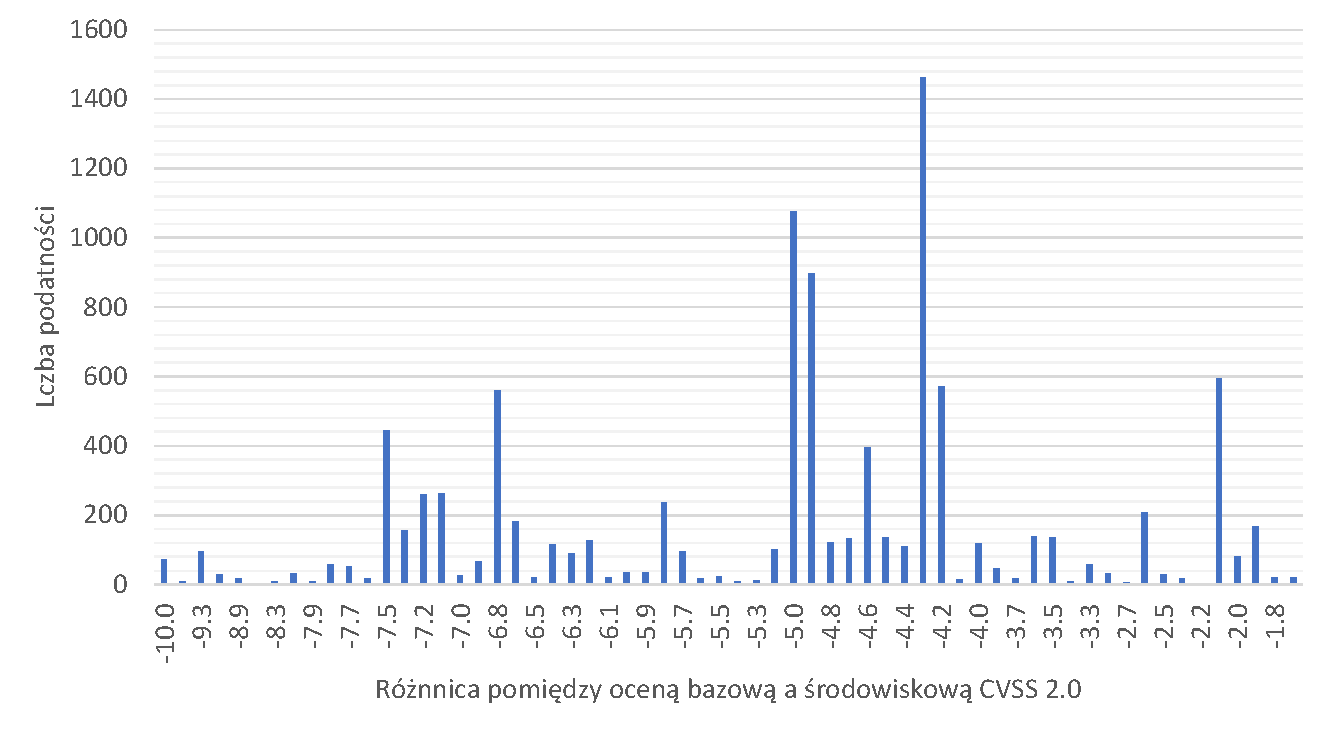
\includegraphics[width=.9\textwidth]{Chapters/Eksperymenty/env_C_results/changes_cvss_2.pdf}
\caption{Liczba podatności zmodyfikowanych dla danej wartości różnicy pomiędzy oceną bazową a środowiskową CVSS 2.0 w przypadku środowiska teleinformatycznego C.}
\label{fig:chapter6:env_c:cvss_2_changes}
\end{figure}

\bigbreak
Tabela \ref{tab:chapter6:env_c:time_results_cvss2} przedstawia liczbę roboczogodzin wymaganą do usunięcia istotnych podatności bezpieczeństwa dla środowiska teleinformatycznego C. W przypadku ocen bazowych CVSS 2.0 szacunkowa liczba roboczogodzin została obliczona za pomocą wzorów: $T_{Base2}$ - \ref{eq:cvss2}, $T_{Base2'}$ - \ref{eq:cvss2prim}. W przypadku oceny środowiskowej CVSS 2.0 szacunkowa liczba roboczogodzin została obliczona za pomocą wzoru \ref{eq:cvss2e}. Wartości dla czasów $T_{Base2}$ obliczone zostały przy założeniu, że administrator musi naprawić tylko podatności o krytyczności wysokiej i średniej, w związku z czym akceptuje ryzyko związane z istnieniem w systemie podatności o krytyczności niskiej. Ponadto należy zauważyć, ze w przypadku priortetyzacji opartej na ocenie bazowej CVSS 2.0, która nie uwzględnia danych środowiskowych wśród podatności sklasyfikowanych jako podatności o krytyczności niskiej, mogą się znajdować podatności o wyższej krytyczności, na przykład wysokiej. Wartości czasów $T_{Base2'}$ obliczone zostały zatem przy założeniu, że w celu zapewnienia bezpieczeństwa systemu administrator musi naprawić wszystkie podatności, ponieważ (jak opisano szczegółowo w rozdziale \ref{sec:wplyw_cvss2}) nie ma pewności czy podatność z otrzymaną oceną bazową CVSS 2.0 zachowa tę ocenę po uwzględnieniu danych środowiskowych. Natomiast wartości dla czasów $T_{Env2}$ obliczone zostały przy założeniu, że wszystkie oceny podatności zostały sklasyfikowane dokładnie (Rozdział \ref{sec:modele-zarzadzaia-podatnosciami}). Gdy porówna się szacowane liczby roboczogodzin otrzymane dla $T_{Base2}$ z $T_{Base2'}$, można zauważyć wzrost szacowanej liczy roboczogodzin dla wszystkich rozpatrywanych przypadków ($T_{FIX_{MIN}}$, $T_{FIX_{AVERAGE}}$, $T_{FIX_{MAX}}$), który wynosi 16.7\%. Ponadto można zaobserwować, że naprawienie wszystkich podatności według otrzymanej priorytetyzacji za pomocą oceny bazowej CVSS 2.0 redukuje ryzyko nienaprawienia podatności niedoszacowanej z 17.8\% do 0\%. Gdy porównamy otrzymane wyniki dla $T_{Base2}$ i $T_{Env2}$, można zauważyć, że średni zysk w postaci obniżenia szacowanej liczby roboczogodzin dla wszystkich rozpatrywanych przypadków wynosi 99.8\%. Wykorzystanie priorytetyzacji za pomocą oceny środowiskowej CVSS 2.0 pozwala na obniżenie ryzyka związanego z nienaprawieniem podatności niedoszacowanej z 17.8\% do 0\%. Natomiast gdy porówna się wyniki otrzymane dla $T_{Base2'}$ i $T_{Env2}$, można zauważyć, że średni zysk w postaci obniżenia szacowanej liczby roboczogodzin dla wszystkich rozpatrywanych przypadków wynosi 99.9\% i tym samym utrzymuje ryzyko związane z nienaprawieniem podatności niedoszacowanych na poziomie 0\%.

\begin{table}[tbh]
\caption{Liczba roboczogodzin wymagana do usunięcia istotnych podatności dla bezpieczeństwa środowiska teleinformatycznego C. W przypadku ocen bazowych CVSS 2.0 szacunkowa liczba roboczogodzin została obliczona za pomocą wzorów: $T_{Base2}$ - \ref{eq:cvss2}, $T_{Base2'}$ - \ref{eq:cvss2prim}. W przypadku oceny środowiskowej CVSS 2.0 szacunkowa liczba roboczogodzin została obliczona za pomocą wzoru \ref{eq:cvss2e}.}
\begin{center}
\label{tab:chapter6:env_c:time_results_cvss2}
\begin{tabular}{c|ccc|c}
\hline
                 & \textbf{$T_{FIX_{MIN}}$} & \textbf{$T_{FIX_{AVERAGE}}$} & \textbf{$T_{FIX_{MAX}}$ }  & Średnia \% zmiana \\
\hline
$T_{Base2}$      &                      8 311h &         37 319h   &  74 615h           &        \\
$T_{Base2'}$     &                     10 101h &         45 374h   &  90 725h           &         \\
Różnica          &           +1 790h (+21.5\%) & +8 055h (+21.6\%) & +16 110h (+21.6\%) & +21.6\%   \\  
\hline
$T_{Base2}$     &                       8 311h &           37 319h &  74 615h        &         \\
$T_{Env2}$        &                        23h &               23h &     23h         &         \\
Różnica          &           -8 288h (-99.7\%) & -37 269h (-99.9\%) & -74 592h (-99.9\%) & -99.8\% \\  
\hline
$T_{Base2'}$     &                      10 101h &       45 374h    &  90 725h        &         \\
$T_{Env2}$        &                        23h &               23h  &     23h        &         \\
Różnica          &           -10 078h (-99.8\%) & -45 351h (-99.9\%) & -90 702h (-99.9\%) & -99.9\% \\  
\hline
\end{tabular}
\end{center}
\end{table}

\bigbreak
Jak wykazano w przeprowadzonej analizie, model zarządzania podatnościami, który wykorzystuje ocenę środowiskową CVSS 2.0, ma istotną wadę. Wada ta polega na tym, że parametr $TD$, który służy do ustalania liczby systemów wrażliwych na daną podatność, znacząco zaniża oceny wszystkich wykrytych podatności. W analizowanym środowisku teleinformatycznym C spowodował sklasyfikowanie wszystkich podatności do kategorii niskiej. Dlatego też ocena środowiskowa CVSS 2.0 nie jest dokładną miarą bezpieczeństwa infrastruktury teleinformatycznej. Analiza wyników pozwala na wyciągnięcie kolejnego wniosku. Mianowicie model zarządzania podatnościami przy zastosowaniu oceny środowiskowej CVSS 2.0 (Rysunek \ref{fig:chapter1:vm-model-cvss2e}) może być wykorzystany do wykrywania podatności, które mogą zagrozić większej liczbie skanowanych zasobów. Taka informacja jest niezwykle cenna dla wszystkich osób zaangażowanych w proces zarządzania podatnościami (Rozdział \ref{sec:proces-zarzadzania-podatnosciami}), ponieważ pozwala na podjęcie szybkiej decyzji dotyczącej naprawy podatności oraz skrócenie czasu ich obecności w monitorowanej infrastrukturze teleinformatycznej.

%%%%%%%%%%%%%%%%%%%%%%%%%%%%%%%%%%%%%%%%%%%%%%%%

%%%%%%%%%%%%%%%%%%%%%%%%%%%%%%%%%%%%%%%%%%%%%%%%
\subsubsection{Analiza wpływu parametrów środowiskowych na ocenę bazową CVSS 3.x}

W celu wykonania analizy wpływu parametrów środowiskowych na ocenę bazową CVSS 3.x rozróżniono dwa przypadki. W pierwszym przypadku rozważane jest wykorzystanie metody konwersji ocen bazowych CVSS 2.0 do 3.x za pomocą uczenia maszynowego. W drugim przypadku rozważane jest brak metod konwersji i dopuszczany jest brak wiedzy na temat wszystkich ocen bazowych CVSS 3.x dla nieznacznej liczby wykrytych podatności.

\bigbreak
Dla pierwszego rozpatrywanego przypadku, w celu zapewnienia poprawnej priorytetyzacji wszystkich podatności za pomocą modeli zarządzania podatnościami wykorzystującymi CVSS 3.x (Rysunki \ref{fig:chapter1:vm-model-cvss3}, \ref{fig:chapter1:vm-model-cvss3e}), wykorzystano mechanizm konwersji CVSS 2.0 do CVSS 3.x za pomocą uczenia maszynowego (Rozdział \ref{sec:ml}, ponieważ 34\% podatności nie posiada oceny bazowej według CVSS 3.x dla środowiska teleinformatycznego C (Rozdział \ref{sec:desc_c}). W tabeli \ref{tab:chapter6:env_c:ml_classification} przedstawiono liczbę zmian dla każdej kategorii podatności według oceny bazowej CVSS 3.x w przypadku środowiska teleinformatycznego C, po zastosowaniu mechanizmu konwersji oceny bazowej CVSS 2.0 do CVSS 3.x (ML) opartego na uczeniu maszynowym. Wykorzystany mechanizm uczenia maszynowego oblicza ocenę bazową CVSS 3.x obarczoną błędem klasyfikacji kategorii krytyczności wynoszącym 3.45\%, co oznacza, że można oczekiwać 48 podatności błędnie sklasyfikowanych w środowisku teleinformatycznym C. W dalszej części podrozdziału skupiono się tylko na analizie wyników przypadku pierwszego dotyczącego prioretetyzacji podatności według oceny środowiskowej CVSS 3.x z wykorzystaniem metod konwersji ocen bazowych CVSS 2.0 do 3.x za pomocą uczenia maszynowego.


\begin{table}[tbh]
\caption{Liczba zmian dla każdej kategorii podatności według oceny bazowej CVSS 3.x w przypadku środowiska teleinformatycznego C po zastosowaniu mechanizmu konwersji oceny bazowej CVSS 2.0 do CVSS 3.x (ML) opartego na uczeniu maszynowym.}
\begin{center}
\label{tab:chapter6:env_c:ml_classification}
\begin{tabular}{cccc}
\hline \noalign {\smallskip}
\textbf{Kategoria} & \textbf{ocena bazowa} & \textbf{[ML] ocena bazowa} & \textbf{Różnica} \\
                      & \textbf{CVSS 3.x} & \textbf{CVSS 3.x} & \\
  \hline
  Niska         &    802 &  996    &  +194          \\
                &        &         &  (+24.1\%)     \\
  Średnia       &  4 453 &   4 511 &  +58           \\
                &        &         &  (+1.3\%)       \\
  Wysoka        &  2 651 &   2 682 &  +31           \\
                &        &         &  (+1.2\%)   \\
  Krytyczna     &  1 824 &  1 889  &  +65          \\
                &        &         &  (+3.6\%)   \\
\hline \noalign {\smallskip}
\textbf{Razem}  &   9 730 &   10 078& +348 \\
                &        &         & (+3.6\%) \\
\hline \noalign {\smallskip}
\end{tabular}
\end{center}
\end{table}

\bigbreak
Rysunek \ref{fig:chapter6:env_c:cvss_3} przedstawia liczbę wykrytych podatności dla każdej kategorii krytyczności według oceny bazowej i środowiskowej CVSS 3.x dla środowiska teleinformatycznego C. Na podstawie wyników pokazanych na rysunku \ref{fig:chapter6:env_a:cvss_3} można stwierdzić znaczącą zmianę w stosunku do oceny bazowej CVSS 3.x, która polega na zmniejszeniu liczby podatności krytycznych oraz wysokich a zwiększeniu liczby podatności o kategorii średniej oraz niskiej. Wpływ na to mają ustawienia wagi zasobów, wskazane przez administratora środowiska teleinformatycznego C o rozkładzie przedstawionym na rysunku \ref{fig:chapter5:env_c:os_cia}. Analiza wpływu parametrów środowiskowych $CIA$ na ocenę bazową CVSS 3.x przedstawiona została w rozdziale 4.

\begin{figure}[!ht]
\centering
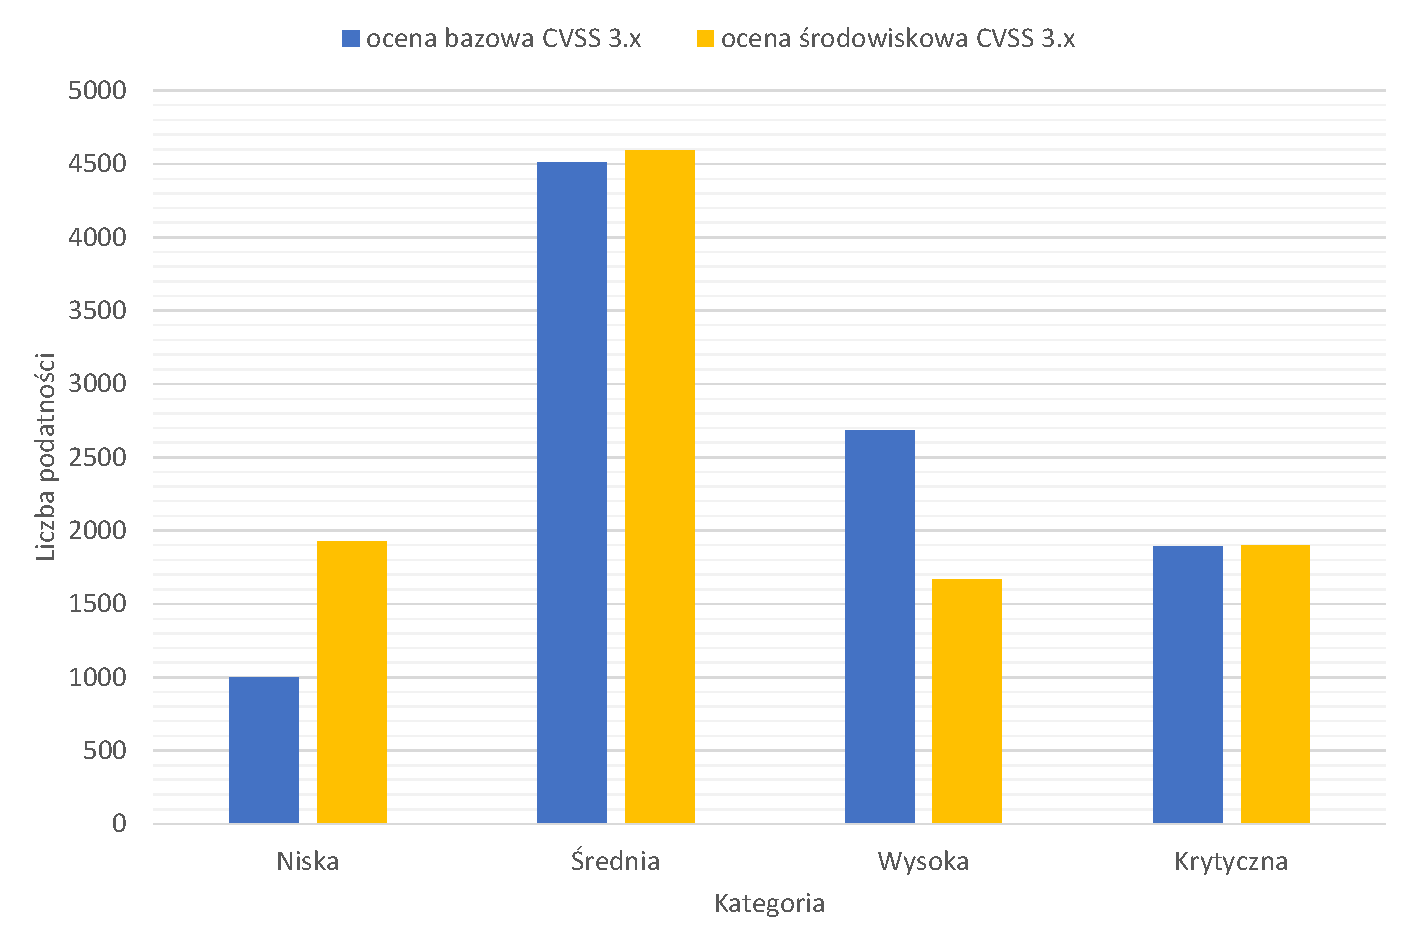
\includegraphics[width=.9\textwidth]{Chapters/Eksperymenty/env_C_results/cvss_3_ml.pdf}
\caption{Liczba wykrytych podatności dla każdej kategorii krytyczności według oceny bazowej i środowiskowej CVSS 3.x dla środowiska teleinformatycznego C.}
\label{fig:chapter6:env_c:cvss_3}
\end{figure}

\bigbreak
Rysunek \ref{fig:chapter6:env_c:cvss_3_changes} przedstawia liczbę wszystkich podatności zmodyfikowanych dla danej wartości różnicy pomiędzy oceną bazową a środowiskową CVSS 3.x w przypadku środowiska teleinformatycznego C. Wyniki przedstawione na rysunku \ref{fig:chapter6:env_c:cvss_3_changes} dotyczą rozpatrywanego przypadku pierwszego, w którym to uwzględnione są podatności z obliczoną oceną bazową CVSS 3.x za pomocą uczenia maszynowego. Parametry środowiskowe $CIA$ dla wskazanych zasobów spowodowały modyfikację  6 121 (60.73\%) ocen bazowych w zakresie od -2.3 do 2.2. Na pozostałe podatności ustawienia parametrów środowiskowych nie miały wpływu.

\begin{figure}[!ht]
\centering
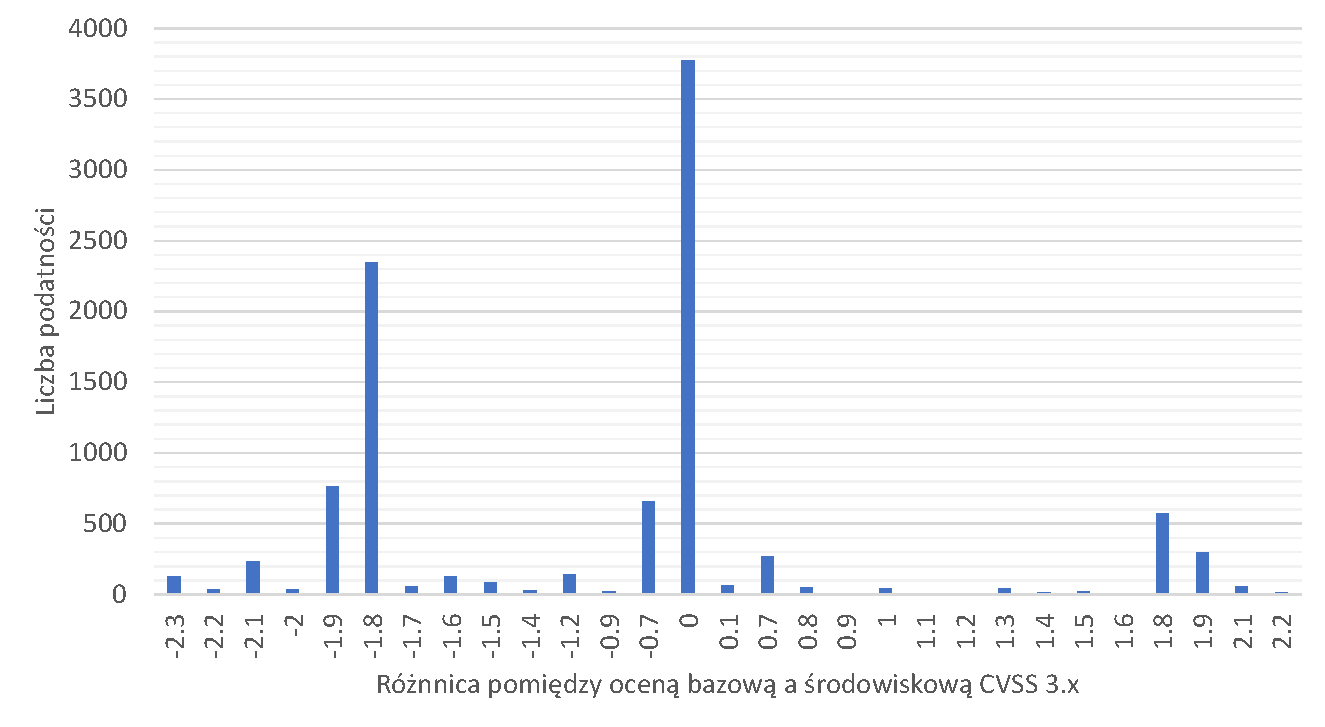
\includegraphics[width=.9\textwidth]{Chapters/Eksperymenty/env_C_results/changes_cvss_3.pdf}
\caption{Liczba wszystkich podatności zmodyfikowanych dla danej wartości różnicy pomiędzy oceną bazową a środowiskową CVSS 3.x w przypadku środowiska teleinformatycznego C.}
\label{fig:chapter6:env_c:cvss_3_changes}
\end{figure}

\bigbreak
Tabela \ref{tab:chapter6:env_c:changes_cvss_3} przedstawia liczbę zmian w kategoriach krytyczności podatności dla środowiska teleinformatycznego C po uwzględnieniu parametrów środowiskowych $CIA$ przy wykorzystaniu metod konwersji oceny bazowej CVSS 2.0 do 3.x za pomocą uczenia maszynowego. Największa zmiana w liczbie podatności została odnotowana dla kategorii krytycznej (+94.58\%) oraz wysokiej (-39.96\%). Dla zasobów posiadających wartości parametrów środowiskowych $CIA$ wykryto 10 023 podatności, co stanowi 99.45\% wszystkich podatności, 21.98\% z nich zmieniło swoją kategorię. Uzyskane wyniki pozwalają na wyciągnięcie dwóch wniosków. Pierwszy mówi o tym, że możliwe jest wykorzystanie mechanizmu konwersji oceny bazowej CVSS 2.0 do 3.x do pełnej implementacji modelu zarządzania podatnościami opartego na ocenie środowiskowej CVSS 3.x dla wszystkich podatności. Natomiast drugi wniosek pozwala na stwierdzenie, że każda dodatkowa informacja na temat monitorowanego środowiska wpływa na priorytetyzacje napraw podatności poprzez możliwość zmiany kategorii krytyczności podatności.

\begin{table}[tbh]
\caption{Liczba zmian w kategoriach podatności dla środowiska teleinformatycznego C z wykorzystaniem metod konwersji oceny bazowej CVSS 2.0 do CVSS 3.x za pomocą uczenia maszynowego.}
\begin{center}
\label{tab:chapter6:env_c:changes_cvss_3}
\begin{tabular}{cccc}
\hline \noalign {\smallskip}
\textbf{Kategoria}  & \textbf{ocena bazowa} & \textbf{ocena środowiskowa} & \textbf{Różnica} \\
                      & \textbf{CVSS 3.x} & \textbf{CVSS 3.x} & \\
\hline \noalign {\smallskip}
  Niska         &   996 &  1 938 &  +942           \\
                &       &        & (+94.58\%)    \\
  Średnia       & 4 511 &  4 592 &  +81            \\
                &       &        & (+1.79\%)      \\
  Wysoka        & 2 682 &  1 664 &  -1018           \\
                &       &        &  (-39.96\%)     \\
  Krytyczna     & 1 889 &  1 884 &  -5           \\
                &       &        &  (-0.26\%)     \\
\hline \noalign {\smallskip}
 \textbf{Razem} & 10 078&  10 078&      2 046 \\
                     &  & &    (20.30\%) \\
\hline \noalign {\smallskip}
\end{tabular}
\end{center}
\end{table}

\bigbreak
Tabela \ref{tab:chapter6:env_c:time_results_cvss3} przedstawia liczbę roboczogodzin wymaganą do usunięcia istotnych podatności bezpieczeństwa dla środowiska teleinformatycznego C. W przypadku ocen bazowych CVSS 3.x szacunkowa liczba roboczogodzin została obliczona za pomocą wzorów: $T_{Base3ML}$ - \ref{eq:cvss3}, $T_{Base3'ML}$ - \ref{eq:cvss3prim}. W przypadku oceny środowiskowej CVSS 3.x szacunkowa liczba roboczogodzin została obliczona za pomocą wzoru \ref{eq:cvss2e}. Wartości dla czasów $T_{Base3ML}$ obliczone zostały przy założeniu, że administrator musi naprawić tylko podatności o krytyczności wysokiej i średniej, w związku z czym akceptuje ryzyko związane z istnieniem w systemie podatności o krytyczności niskiej. Ponadto należy zauważyć, ze w przypadku priortetyzacji opartej na ocenie bazowej CVSS 3.x, która nie uwzględnia danych środowiskowych wśród podatności sklasyfikowanych jako podatności o krytyczności niskiej, mogą się znajdować podatności o wyższej krytyczności, na przykład wysokiej. Wartości czasów $T_{Base3'ML}$ obliczone zostały zatem przy założeniu, że w celu zapewnienia bezpieczeństwa systemu administrator musi naprawić wszystkie podatności, ponieważ (jak opisano szczegółowo w rozdziale \ref{sec:wplyw_cvss3}) nie ma pewności, czy podatność z otrzymaną oceną bazową CVSS 3.x zachowa tę ocenę po uwzględnieniu danych środowiskowych. Natomiast wartości dla czasów $T_{Env3ML}$ obliczone zostały przy założeniu, że wszystkie oceny podatności zostały sklasyfikowane dokładnie (Rozdział \ref{sec:modele-zarzadzaia-podatnosciami}). Gdy porówna się szacowane liczby roboczogodzin otrzymane dla $T_{Base3ML}$ z $T_{Base3ML'}$, można zauważyć wzrost szacowanej liczy roboczogodzin dla wszystkich rozpatrywanych przypadków ($T_{FIX_{MIN}}$, $T_{FIX_{AVERAGE}}$, $T_{FIX_{MAX}}$), który wynosi 11\%. Ponadto można zaobserwować, że naprawienie wszystkich podatności według otrzymanej priorytetyzacji za pomocą oceny bazowej CVSS 3.x redukuje ryzyko nienaprawienia podatności niedoszacowanej z 19.9\% do 0.5\%. Gdy porównamy otrzymane wyniki dla $T_{Base3ML}$ i $T_{Env3ML}$, można zauważyć, że średni zysk w postaci obniżenia szacowanej liczby roboczogodzin dla wszystkich rozpatrywanych przypadków wynosi 10.4\%. Wykorzystanie priorytetyzacji za pomocą oceny środowiskowej CVSS 3.x pozwala na obniżenie ryzyka związanego z nienaprawieniem podatności niedoszacowanej z 9.9\% do 0.5\%. Natomiast gdy porówna się wyniki otrzymane dla $T_{Base3'ML}$ i $T_{Env3ML}$, można zauważyć, że średni zysk w postaci obniżenia szacowanej liczby roboczogodzin dla wszystkich rozpatrywanych przypadków wynosi 19.2\% i tym samym utrzymuje ryzyko związane z nienaprawieniem podatności niedoszacowanych na poziomie 0.5\%.

\begin{table}[tbh]
\caption{Liczba roboczogodzin wymagana do usunięcia istotnych podatności bezpieczeństwa dla środowiska teleinformatycznego C. W przypadku ocen bazowych CVSS 3.x szacunkowa liczba roboczogodzin została obliczona za pomocą wzorów: $T_{Base3}$ - \ref{eq:cvss3}, $T_{Base3'}$ - \ref{eq:cvss2prim}. W przypadku oceny środowiskowej CVSS 3.x szacunkowa liczba roboczogodzin została obliczona za pomocą wzoru \ref{eq:cvss3e}.}
\begin{center}
\label{tab:chapter6:env_c:time_results_cvss3}
\begin{tabular}{c|ccc|c}
\hline
                 & \textbf{$T_{FIX_{MIN}}$} & \textbf{$T_{FIX_{AVERAGE}}$} & \textbf{$T_{FIX_{MAX}}$ }  & Średnia \% zmiana \\
\hline
$T_{Base3ML}$    &                        9 105h &           40 892h &    81 761h         &         \\
$T_{Base3'ML}$&                          10 101h &           45 374h &    90 725h         &         \\
Różnica          &               +996h (+10.9\%) &   +4 482h (+11\%) & +8 964h (+11\%) & +11\% \\  
\hline
$T_{Base3ML}$    &                     9 105h &            40 892h &    81 761h         &         \\
$T_{Env3ML}$     &                     8 163h &            36 653h &    73 283h        &         \\
Różnica          &               -942h (-10.3\%)  &  -4 239h (-10.4\%) & -8 478h (-10.4\%) & -10.4\% \\  
\hline
$T_{Base3'ML}$   &                      10 101h &          45 374h &    90 725h         &         \\
$T_{Env3ML}$     &                      8 163h &           36 653h &    73 283h        &         \\
Różnica          &                -1 938h (-19.2\%) & -8 721h (-19.2\%) & -17 442h (-19.2\%) & -19.2\% \\  
\hline
\end{tabular}
\end{center}
\end{table}


\bigbreak
Jak wykazano w przeprowadzonej analizie, parametry środowiskowe $CIA$ mają znaczący wpływ na prioretetyzacje podatności bezpieczeństwa infrastruktury teleinformatycznej. Parametry środowiskowej $CIA$ mają bezpośredni przekład na szacowaną liczbę roboczogodzin wymaganą do poprawy bezpieczeństwa środowiska teleinformatycznego C w procesie zarządzania podatnościami (Rozdział \ref{sec:proces-zarzadzania-podatnosciami}). Wykorzystanie modelu zarządzania podatnościami opartego na ocenie środowiskowej CVSS 3.x (Rysunek \ref{fig:chapter1:vm-model-cvss3e}) z metodami konwersji oceny bazowej CVSS 2.0 do 3.x pozwala na lepsze dopasowanie oceny podatności dla otrzymanych danych opisanych w rozdziale \ref{sec:desc_c}. Jak wynika z przeprowadzonej analizy, możliwe jest otrzymanie wyników oceny środowiskowej niezwłocznie po zakończonym procesie skanowania, co w rezultacie daje zysk w postaci obniżenia szacowanej liczby roboczogodzin na poziomie 19\%, co w najgorszym rozpatrywanym przypadku ($T_{FIX_{MAX}}$) wynosi 17 442 roboczogodzin dla jednej osoby.

%%%%%%%%%%%%%%%%%%%%%%%%%%%%%%%%%%%%%%%%%%%%%%%%

%%%%%%%%%%%%%%%%%%%%%%%%%%%%%%%%%%%%%%%%%%%%%%%%
\subsubsection{Podsumowanie wyników analizy dla środowiska C}
Na podstawie wyników przedstawionych w podrozdziale ''Analiza wpływu parametrów środowiskowych na ocenę bazową CVSS 2.0'' można stwierdzić, że dla oceny środowiskowej wszystkie podatności zostały przydzielone do kategorii niskiej. Wpływ na to ma parametr $TD$, który osiągnął maksymalną wartość 3\%. Dodatkowo z analizy otrzymanych wyników można stwierdzić, że dodanie do oceny bazowej CVSS 2.0 danych środowiskowych powoduje znaczącą redukcje szacowanej liczby roboczogodzin wymaganą do usunięcia istotnych podatności wykrytych w środowisku teleinformatycznym C. Gdy porównamy wyniki otrzymane dla oceny bazowej CVSS 2.0 ($T_{Base2}$) z oceną środowiskową CVSS 2.0 ($T_{Env2}$), można zauważyć, że średni zysk w postaci obniżenia szacowanej liczby roboczogodzin wynosi 99.9\%. Wykorzystanie priorytetyzacji za pomocą oceny środowiskowej CVSS 2.0 pozwala na obniżenie ryzyka związanego z nienaprawieniem podatności niedoszacowanej z 17.8\% do 0\%. Wyniki przedstawione w podrozdziale ''Analiza wpływu parametrów środowiskowych na ocenę bazową CVSS 2.0'' potwierdzają wadę oceny środowiskowej CVSS 2.0 polegającą na tym, że parametr $TD$, który służy do ustalania liczby systemów wrażliwych na daną podatność, znacząco zaniża oceny wszystkich podatności. Dlatego konieczne było rozważenie modelu zarządzania podatnościami, który opiera się na standardzie CVSS 3.x.

\bigbreak
Na podstawie wyników przedstawionych w podrozdziale ''Analiza wpływu parametrów środowiskowych na ocenę bazową CVSS 3.x'; można stwierdzić, że wykorzystany mechanizm uczenia maszynowego wykonał obliczenia dla 3.45\% podatności wykrytych w środowisku teleinformatycznym C, które nie posiadają oceny bazowej CVSS 3.x z błędem klasyfikacji kategorii krytyczności wynoszącym 14\%, co oznacza, że można oczekiwać 48 podatności błędnie sklasyfikowanych. Pozwala to na pełną implementację modelu zarządzania podatnościami opartego na standardzie CVSS 3.x (Rysunki \ref{fig:chapter1:vm-model-cvss3}, \ref{fig:chapter1:vm-model-cvss3e}). Z analizy otrzymanych wyników można także stwierdzić, że wpływ parametrów środowiskowych $CIA$ spowodował zmianę kategorii krytyczności dla 20.30\% podatności, co ma bezpośredni przekład na szacowaną liczbę roboczogodzin potrzebną do usunięcia istotnych podatności wykrytych w środowisku teleinformatycznym C. Gdy porównamy wyniki otrzymane dla oceny bazowej CVSS 3.x ($T_{Base3ML}$) z oceną środowiskową CVSS 3.x ($T_{Env3ML}$), można zauważyć redukcję szacowanej liczby roboczogodzin o 10.4\%. Redukcja szacowanej liczby roboczogodzin wynika z lepszego dopasowania kategorii podatności do monitorowanego środowiska teleinformatycznego C (Rozdział \ref{sec:modele-zarzadzaia-podatnosciami}).

%%%%%%%%%%%%%%%%%%%%%%%%%%%%%%%%%%%%%%%%%%%%%%%%

%%%%%%%%%%%%%%%%%%%%%%%%%%%%%%%%%%%%%%%%%%%%%%%%
